\chapter{Falling and Landing Motion Control for Virtual Characters}

\graphicspath{{landing/}}

\begin{figure}[ht]
\center
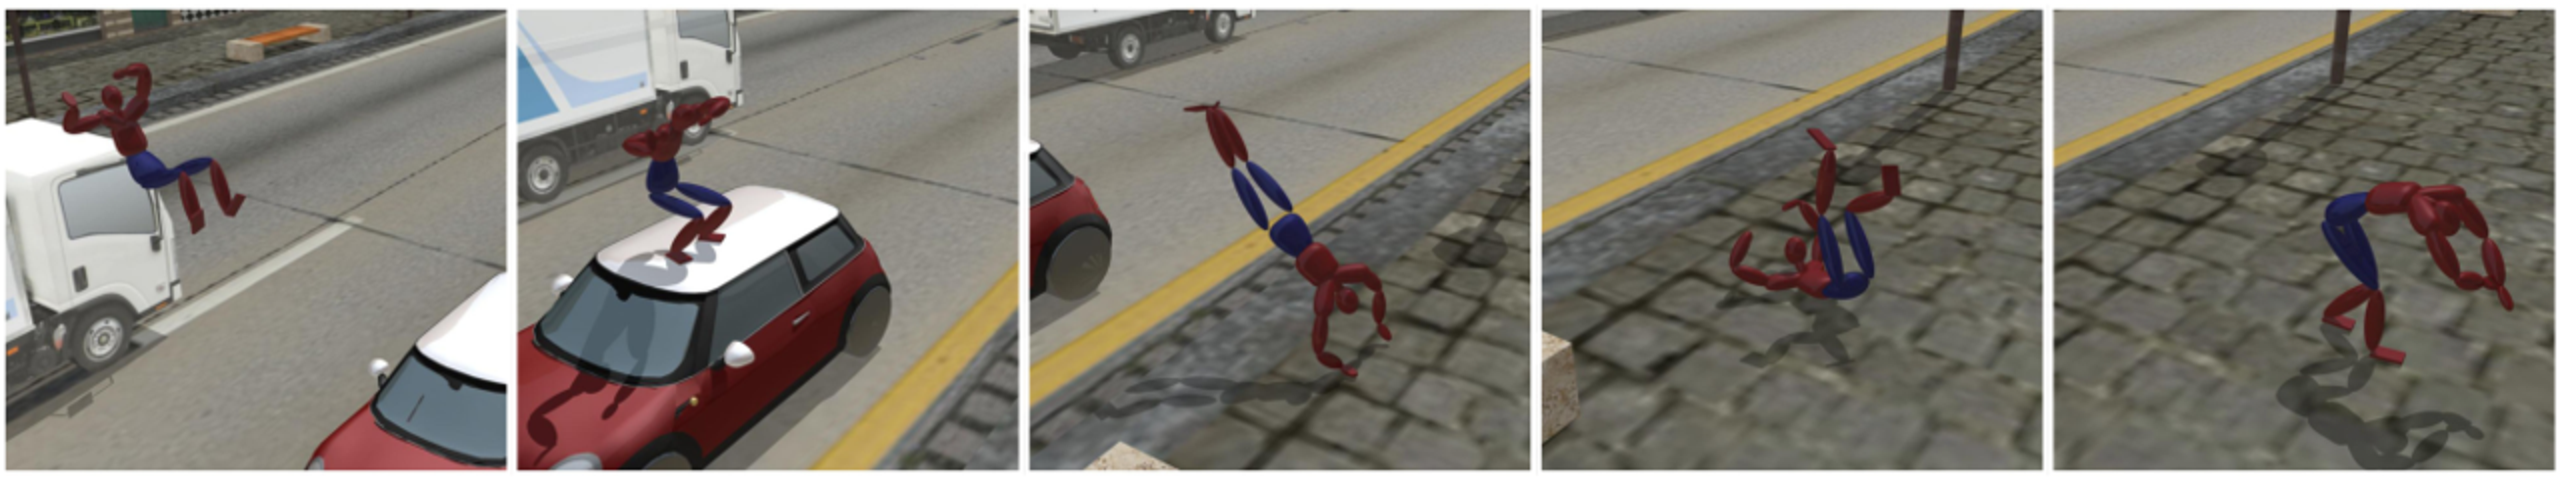
\includegraphics[width=\textwidth]{images/teaser2}
  \caption{A simulated character lands on the roof of a car, leaps
    forward, dive-rolls on the sidewalk, and gets back on its feet,
    all in one continuous motion.}
  \label{fig:landing_teaser}
\end{figure}

This chapter introduces 
a new method to generate agile and natural human landing
motions in real-time via physical simulation without using any mocap
or pre-scripted sequences. We develop a general controller that allows
the character to fall from a wide range of heights and initial speeds,
continuously roll on the ground, and get back on its feet, without
inducing large stress on joints at any moment. The character's motion
is generated through a forward simulator and a control algorithm that
consists of an airborne phase and a landing phase. During the airborne
phase, the character optimizes its moment of inertia to meet the ideal
relation between the landing velocity and the angle of attack, under
the laws of conservation of momentum. The landing phase can be divided
into three stages: impact, rolling, and getting-up. To reduce joint
stress at landing, the character leverages contact forces to control
linear momentum and angular momentum, resulting in a rolling motion
which distributes impact over multiple body parts. We demonstrate that
our control algorithm can be applied to a variety of initial
conditions with different falling heights, orientations, and linear
and angular velocities. Simulated results show that our algorithm can
effectively create realistic action sequences comparable to real world
footage of experienced freerunners.
\section{Motivation}
One of the great challenges in computer animation is to physically
simulate a virtual character performing highly dynamic motion with
agility and grace. A wide variety of athletic movements, such as
acrobatics or freerunning (parkour), involve frequent transitions
between airborne and ground-contact phases. How to land properly to
break a fall is therefore a fundamental skill athletes must acquire. A
successful landing should minimize the risk of injury and disruption
of momentum because the quality of performance largely depends on the
athlete's ability to safely absorb the shock at landing, while
maintaining readiness for the next action. To achieve a successful
landing, the athlete must plan coordinated movements in the air,
control contacting body parts at landing, and execute fluid
follow-through motion. The basic building blocks of these motor skills
can be widely used in other sports that involve controlled falling and
rolling, such as diving, gymnastics, judo, or wrestling.

We introduce a new method to generate agile and natural human
falling and landing motions in real-time via physical simulation
without using motion capture data or pre-scripted animation (Figure
\ref{fig:landing_teaser}). We develop a general controller that allows the
character to fall from a wide range of heights and initial speeds,
continuously roll on the ground, and get back on its feet, without
inducing large stress on joints at any moment. Previous controllers
for acrobat-like motions either precisely define the sequence of
actions and contact states in a state-machine structure, or directly
track a specific motion capture sequence. Both cases fall short of
creating a generic controller capable of handling a wide variety of
initial conditions, overcoming drastic perturbations in runtime, and
exploiting unpredictable contacts.

Our method is inspired by three landing principles informally
developed in freerunning community. First, reaching the ground with
flexible arms or legs provides “cushion” time to dissipate energy over
a longer time window rather than absorbing it instantly at impact. It
also protects the important and fragile body parts, such as the head,
the pelvis, and the tailbone. Second, it is advisable to distribute
the landing impact over multiple body parts to reduce stress on any
particular joint. Third, it is crucial to utilize the friction force
generated by landing impact to steer the forward direction and control
the angular momentum for rolling, a technique referred to as
"blocking" in the freerunning community. These three principles
outline the most commonly employed landing strategy in practice:
landing with feet or hands as the first point of contact, gradually
lowering the center of mass (COM) to absorb vertical impact, and
turning a fall into a roll on the ground, with the head tightly tucked
at impact moment.

However, translating these principles to control algorithms in
a physical simulation is very challenging. During airborne, the
controller needs to plan and achieve the desired first point of
contact and the angle of attack, in the absence of control over the
characters global motion in the air. Instead of solving a large,
nonconvex two-point boundary value problem, we develop a compact
abstract model which can be simulated efficiently for real-time
applications. To strike the balance between accuracy and efficiency,
our algorithm replans the motion frequently to compensate the
approximation due to the simplicity of the model. When the character
reaches the ground, the controller needs to take a series of
coordinated actions involving active changes of contact points over
a large area of human body. Our algorithm executes three consecutive
stages, impact, rolling, and getting-up by controlling poses,
momentum, and contacts at key moments. Furthermore, the airborne and
landing phases are interrelated and cannot be considered in
isolation: the condition for a successful landing defines the
control goals for the airborne phase while the actions taken during
airborne directly impact the landing motion. We approach this
problem in a reverse order of the action sequence: designing a
robust landing controller, deriving a successful landing condition
from this controller, and developing an airborne controller to achieve
the landing condition.


We demonstrate that our control algorithm is general,
efficient, and robust. We apply our algorithm to a variety of
initial conditions with different falling heights, orientations, and
linear and angular velocities. Because the motion is simulated in
real-time, users can apply perturbation forces to alter the course
of the character in the air. Our algorithm is able to efficiently
update the plan for landing given the new situations. We also
demonstrate different strategies to absorb impact, such as a dive
roll, a forward roll, or tumbling. The same control algorithm can be
applied to characters with very different body structures and mass
distributions. We show that a character with unusual body shape can
land and roll successfully.  
Finally, our experiments empirically showed that the algorithm induces
smaller joint stress, except for the contacting end-effectors. In
the worst case of our experiments, the average joint stress is still
four times lower than landing as a passive ragdoll.




\section{Overview}

We introduce a physics-based technique to simulate strategic falling
and landing motions from a wide range of initial conditions. Our
control algorithm reduces joint stress due to landing impact and
allows the character to efficiently recover from the fall. The
character's motion is generated through a forward simulator and a
control algorithm that consists of an \emph{airborne phase} and a
\emph{landing phase}. These two phases are related by an appropriate
\emph{landing strategy}, which describes the body parts used for the
first contact with the ground, a desired landing pose, and an ideal
landing condition that describes the relation between landing
velocities and the angle of attack in successful landing motions. We
develop two most common types of landing strategies: hands-first and
feet-first, and introduce a sampling method to derive the ideal
landing condition for each strategy.

\begin{figure}
\center
  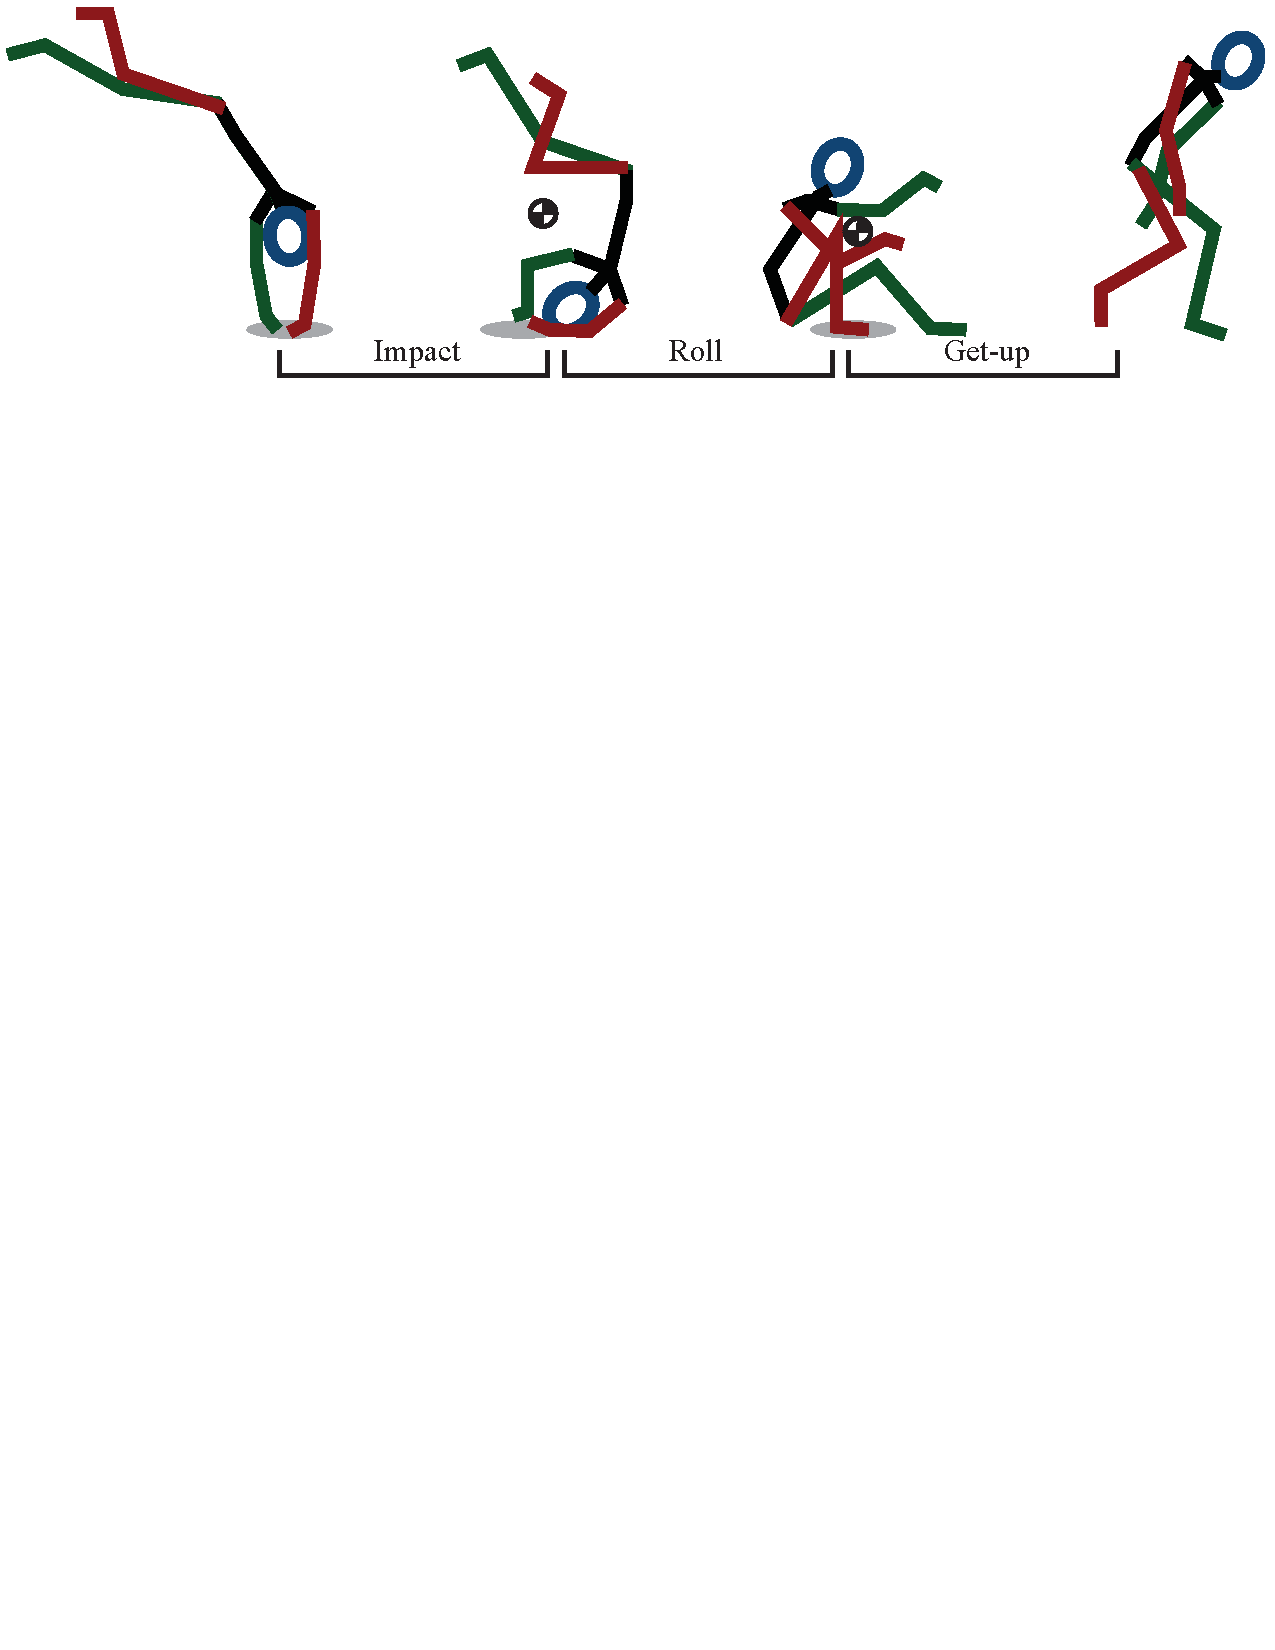
\includegraphics[width=4.2in]{images/landingPhase}
  \caption{Three stages in the landing phase.}
 \label{fig:landing_landingPhase}
\end{figure}

At the beginning of a fall, the character first decides on a landing
strategy. During the airborne phase, the character optimizes its
moment of inertia to achieve the ideal landing condition. The landing
phase is divided into three stages: impact, rolling, and getting-up
(Figure \ref{fig:landing_landingPhase}). The impact stage begins when the
character reaches the ground. 
%% During the impact stage, the character tries to control its linear 
%% and angular momentum while getting into a ready-to-roll pose. 
During the impact stage, the character leverages the friction forces 
from the ground to control linear and angular momentum. 
After the COM moves beyond the hand contact area,
the character switches to the rolling stage in which continuous change
of contact carries out. In preparation for standing up, the character
needs to maintain the rolling direction and plant its feet on the
ground. When the COM passes through the first foot, the character
starts to elevate the COM in order to compete the landing process in an
upright position.

\section{Landing Strategy}

Given an initial condition at the beginning of a fall, the character
can choose to land with the hands-first strategy or the feet-first
strategy.  In general, the hands-first strategy is chosen only for
aesthetics purpose because it is less robust and suitable only for
falls with planar angular momentum (about the pitch axis). In
contrast, the feet-first strategy can handle a wide range of arbitrary
initial conditions because it includes an extensive foot-ground
contact duration to modulate the momentum before rolling. A
landing strategy also includes a desired landing pose. Our algorithm
only requires a partial pose to stretch the arms or legs at landing,
depending on whether the hands-first or the feet-first strategy is
chosen. We manually specify this partial pose for each strategy
(\figref{landing_landingPoses}).


\begin{figure}[ht]
\center
  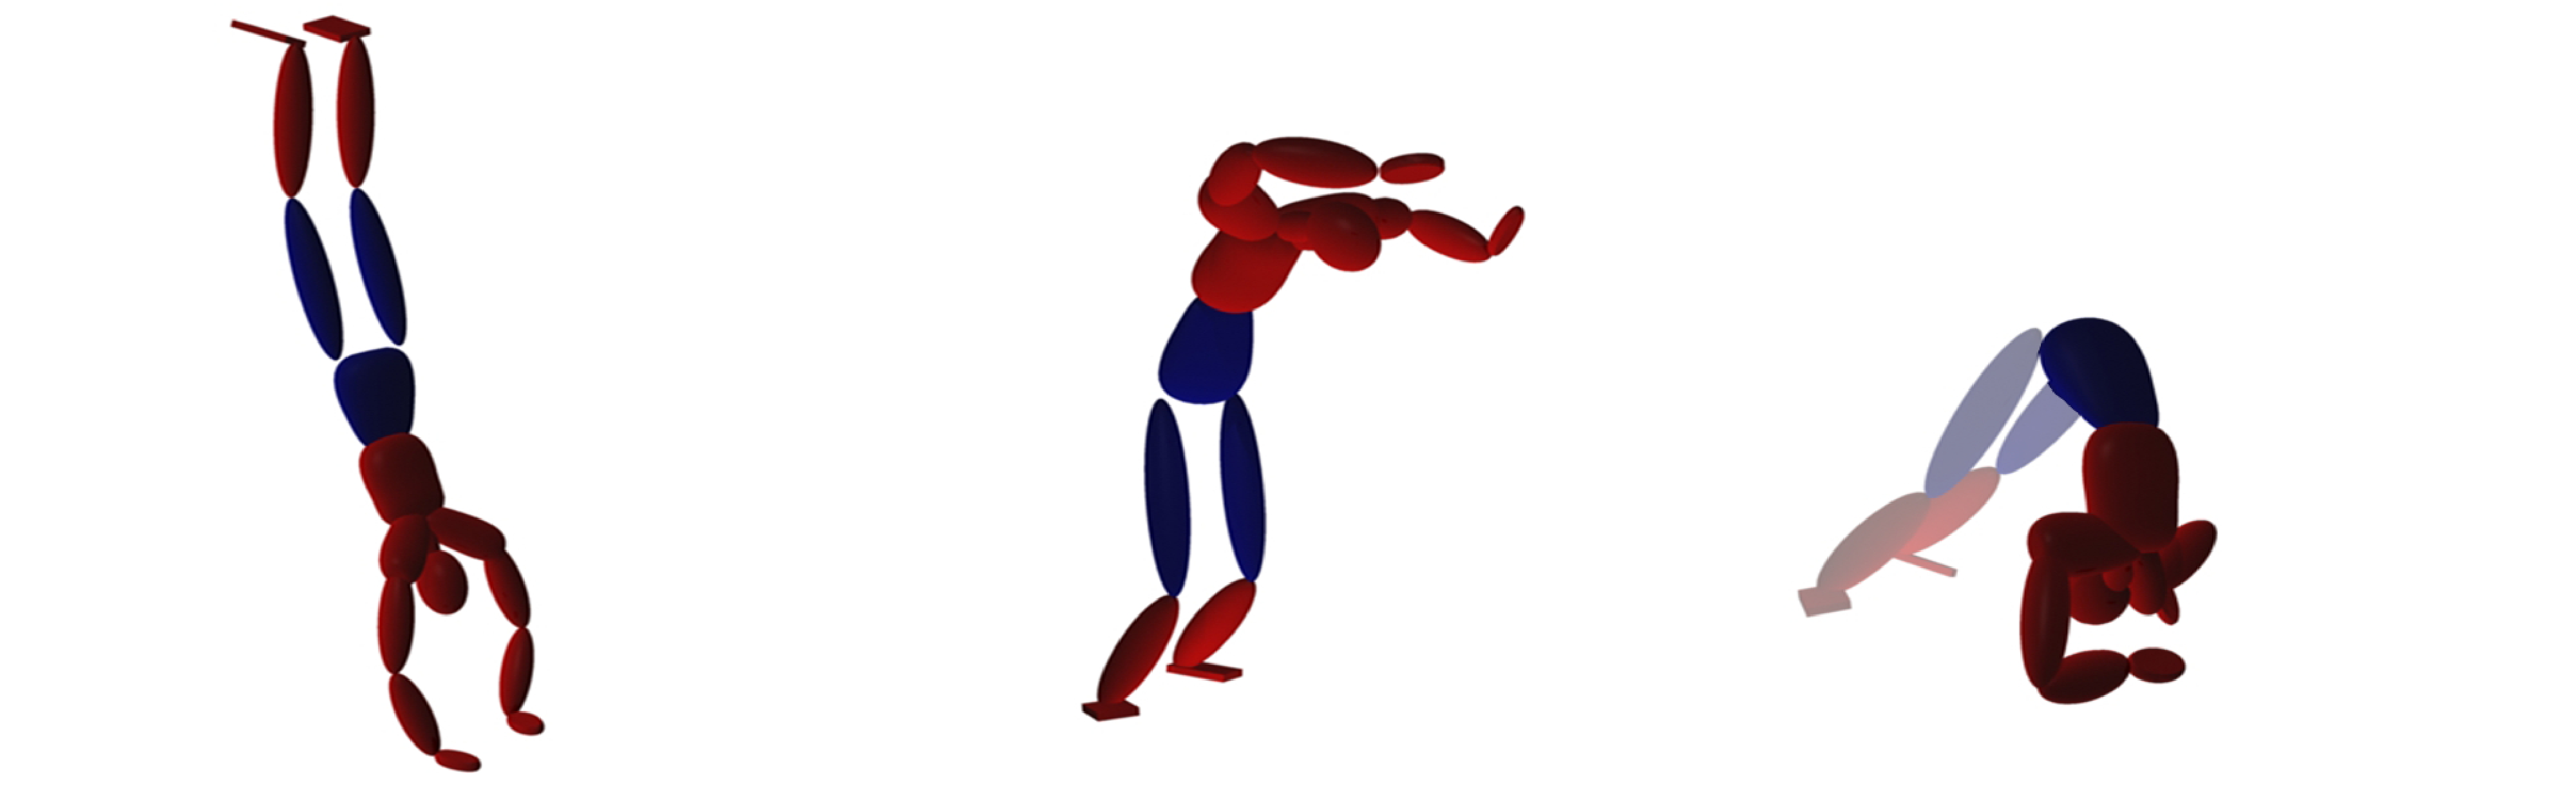
\includegraphics[width=3.2in]{images/LandingPoses}
  \caption{
    The left and middle are the desired landing poses for the
    hands-first strategy and the feet-first strategy, respectively.
    The right is the ready-to-roll pose for the feet-first strategy,
    which we track only the upper body.
  }
 \label{fig:landing_landingPoses}
\end{figure}

\begin{wrapfigure}{l}{0.5\textwidth}
  \begin{center}
    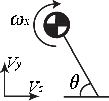
\includegraphics[width=0.28\textwidth]{images/COM}
  \end{center}
  \caption{\revised{Landing condition variables.}}
  \label{fig:landing_com}
\end{wrapfigure}

An integral part of our landing strategy is the landing condition, a
simple equation that compactly characterizes successful landing
motions.
\ignorethis{ A landing strategy describes an ideal landing
  condition key to the success of the subsequent rolling motion. We
  wish to derive a simple equation that compactly characterizes
  successful landing motions.} If the character manages to turn a fall
into a roll and gets back on its feet at the end of the roll, we
consider it successful.  Because a successful landing highly depends
on whether the character is able to control the momentum
at the moment of the first contact ($T$),
%% the character's momentum at the moment of first contact ($T$), 
our algorithm defines the landing condition as a relation between the
global linear velocity $\vc{v}^{(T)}$, global angular velocity
$\vc{\omega}^{(T)}$, and the angle of attack $\theta^{(T)}$, which
approximates the global orientation of the character
(\revised{\figref{landing_com}}).
The actual
coefficients of the landing condition depend on the design of the
landing controller, which cannot be derived analytically, but can be
learned from examples generated by the landing controller. We apply a
sampling method, similar in spirit to the approach Coros \etal
\cite{Coros:2009:RTC} presented for biped locomotion, to determine the
landing condition for a particular landing strategy.  \ignorethis{ A
  successful landing also depends on the design of the landing
  controller, which cannot be expressed in an analytical form.
  Therefore, we use a sampling approach to derive the relation,
  similar in spirit to the approach Coros \etal \cite{Coros:2009:RTC}
  presented for biped locomotion.}

\begin{figure}[ht]
\center
  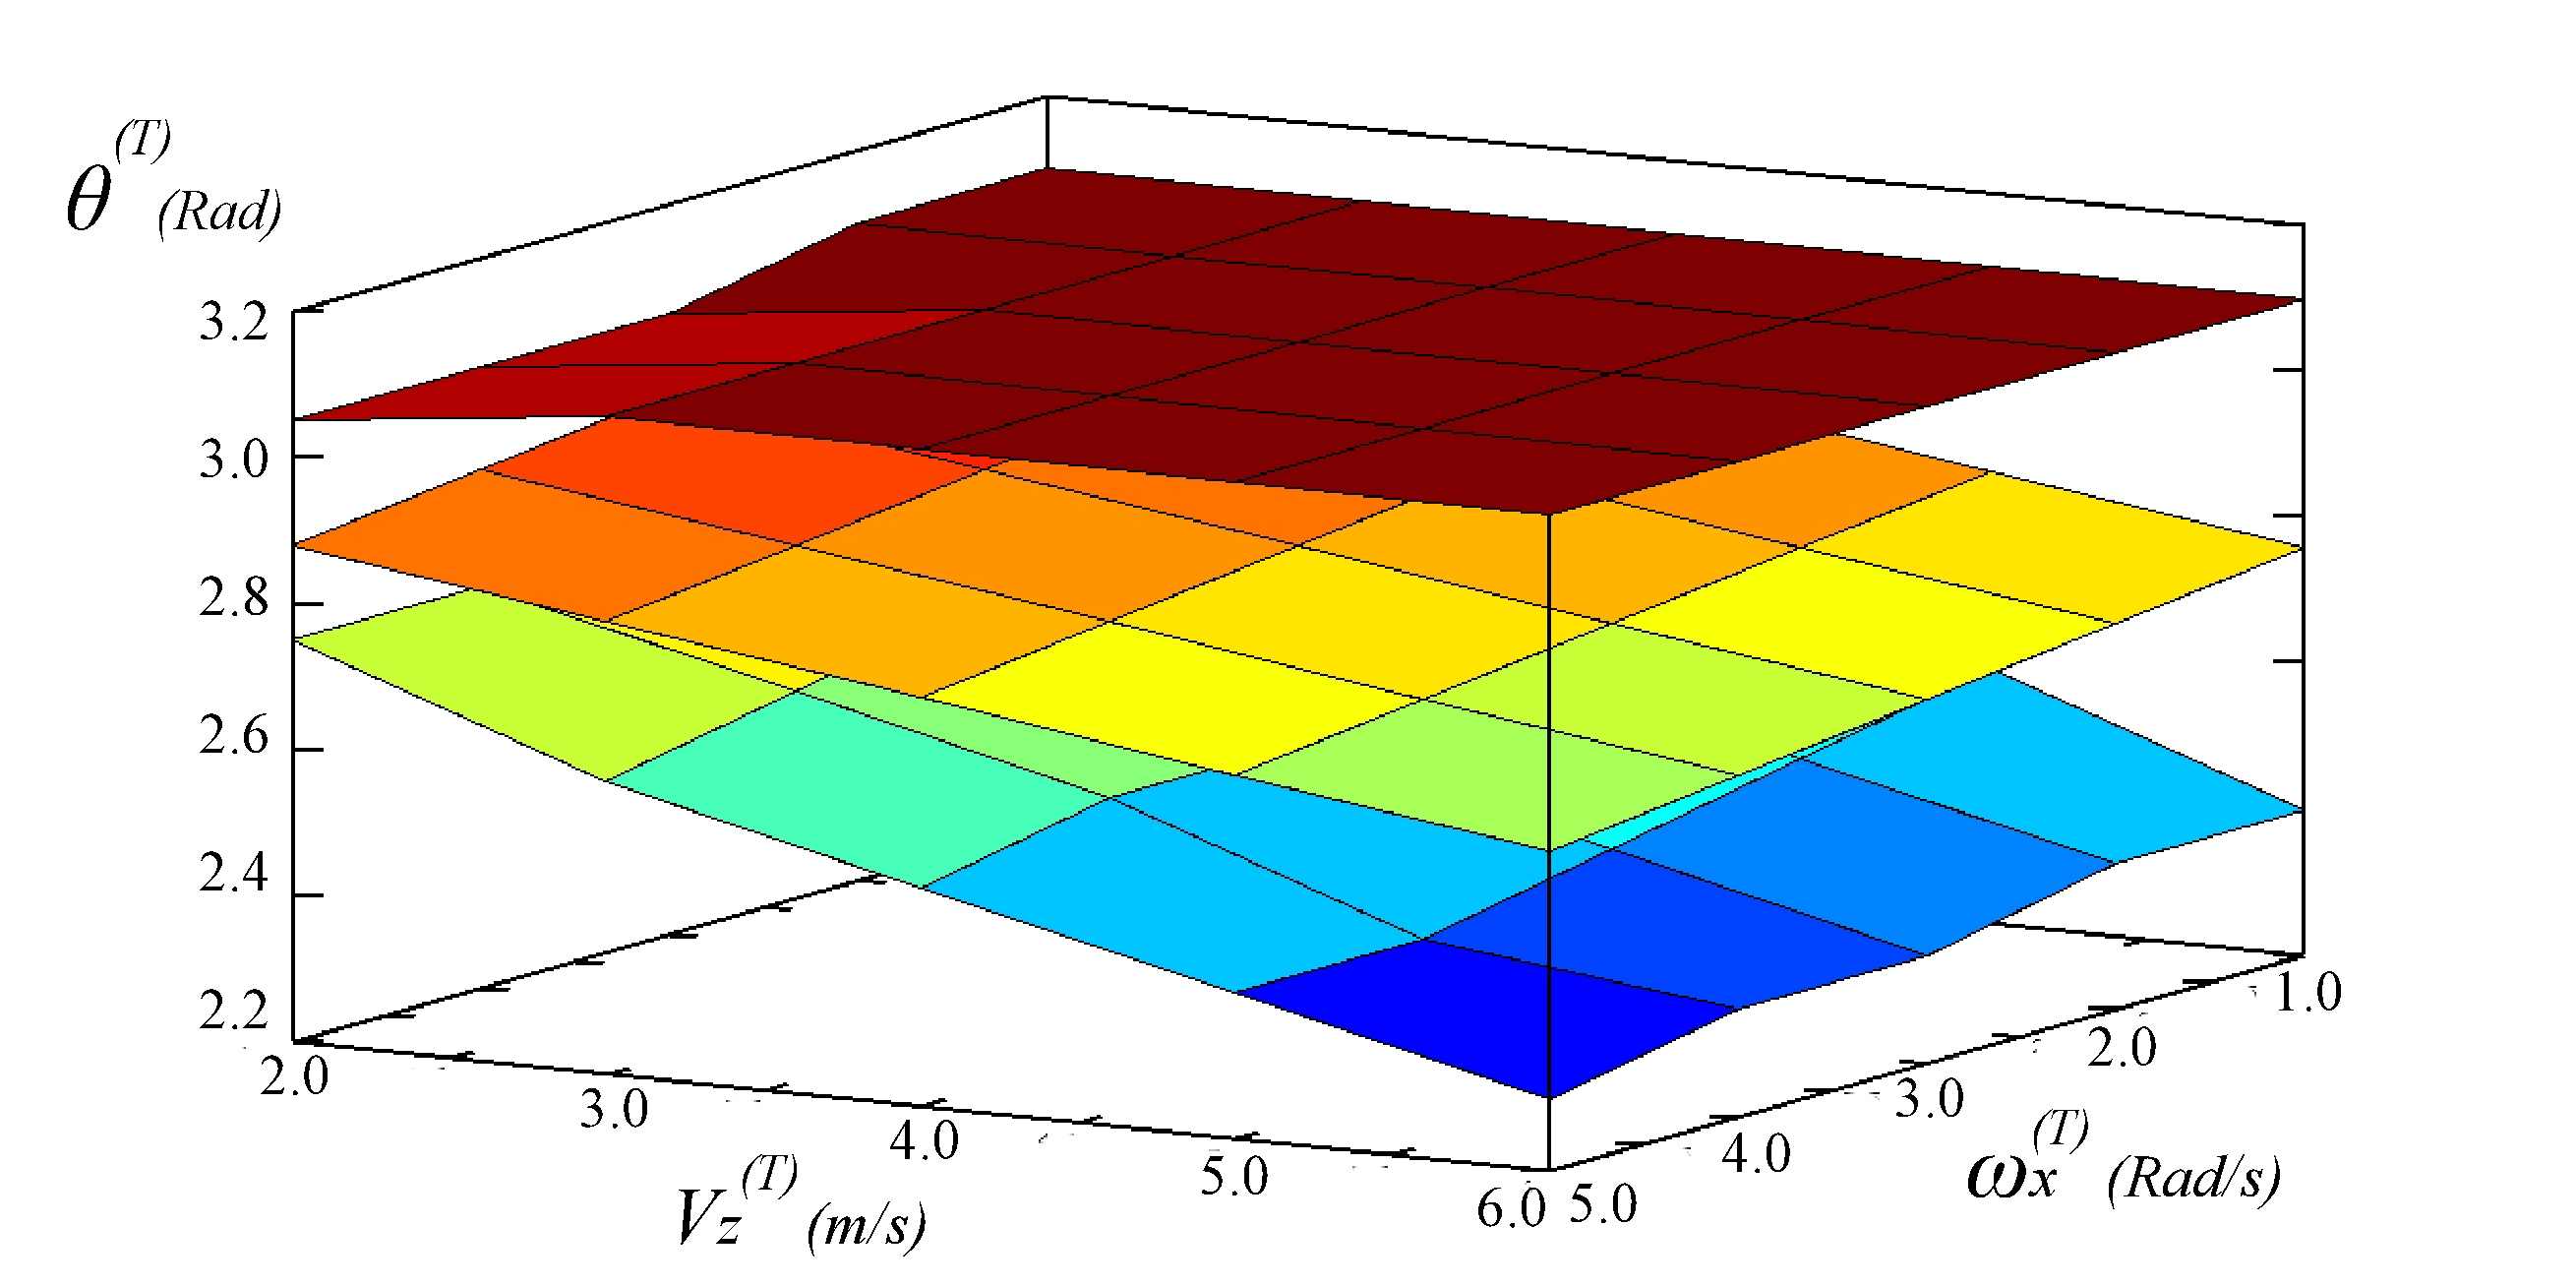
\includegraphics[width=0.49\textwidth]{images/sampleVZWX}
  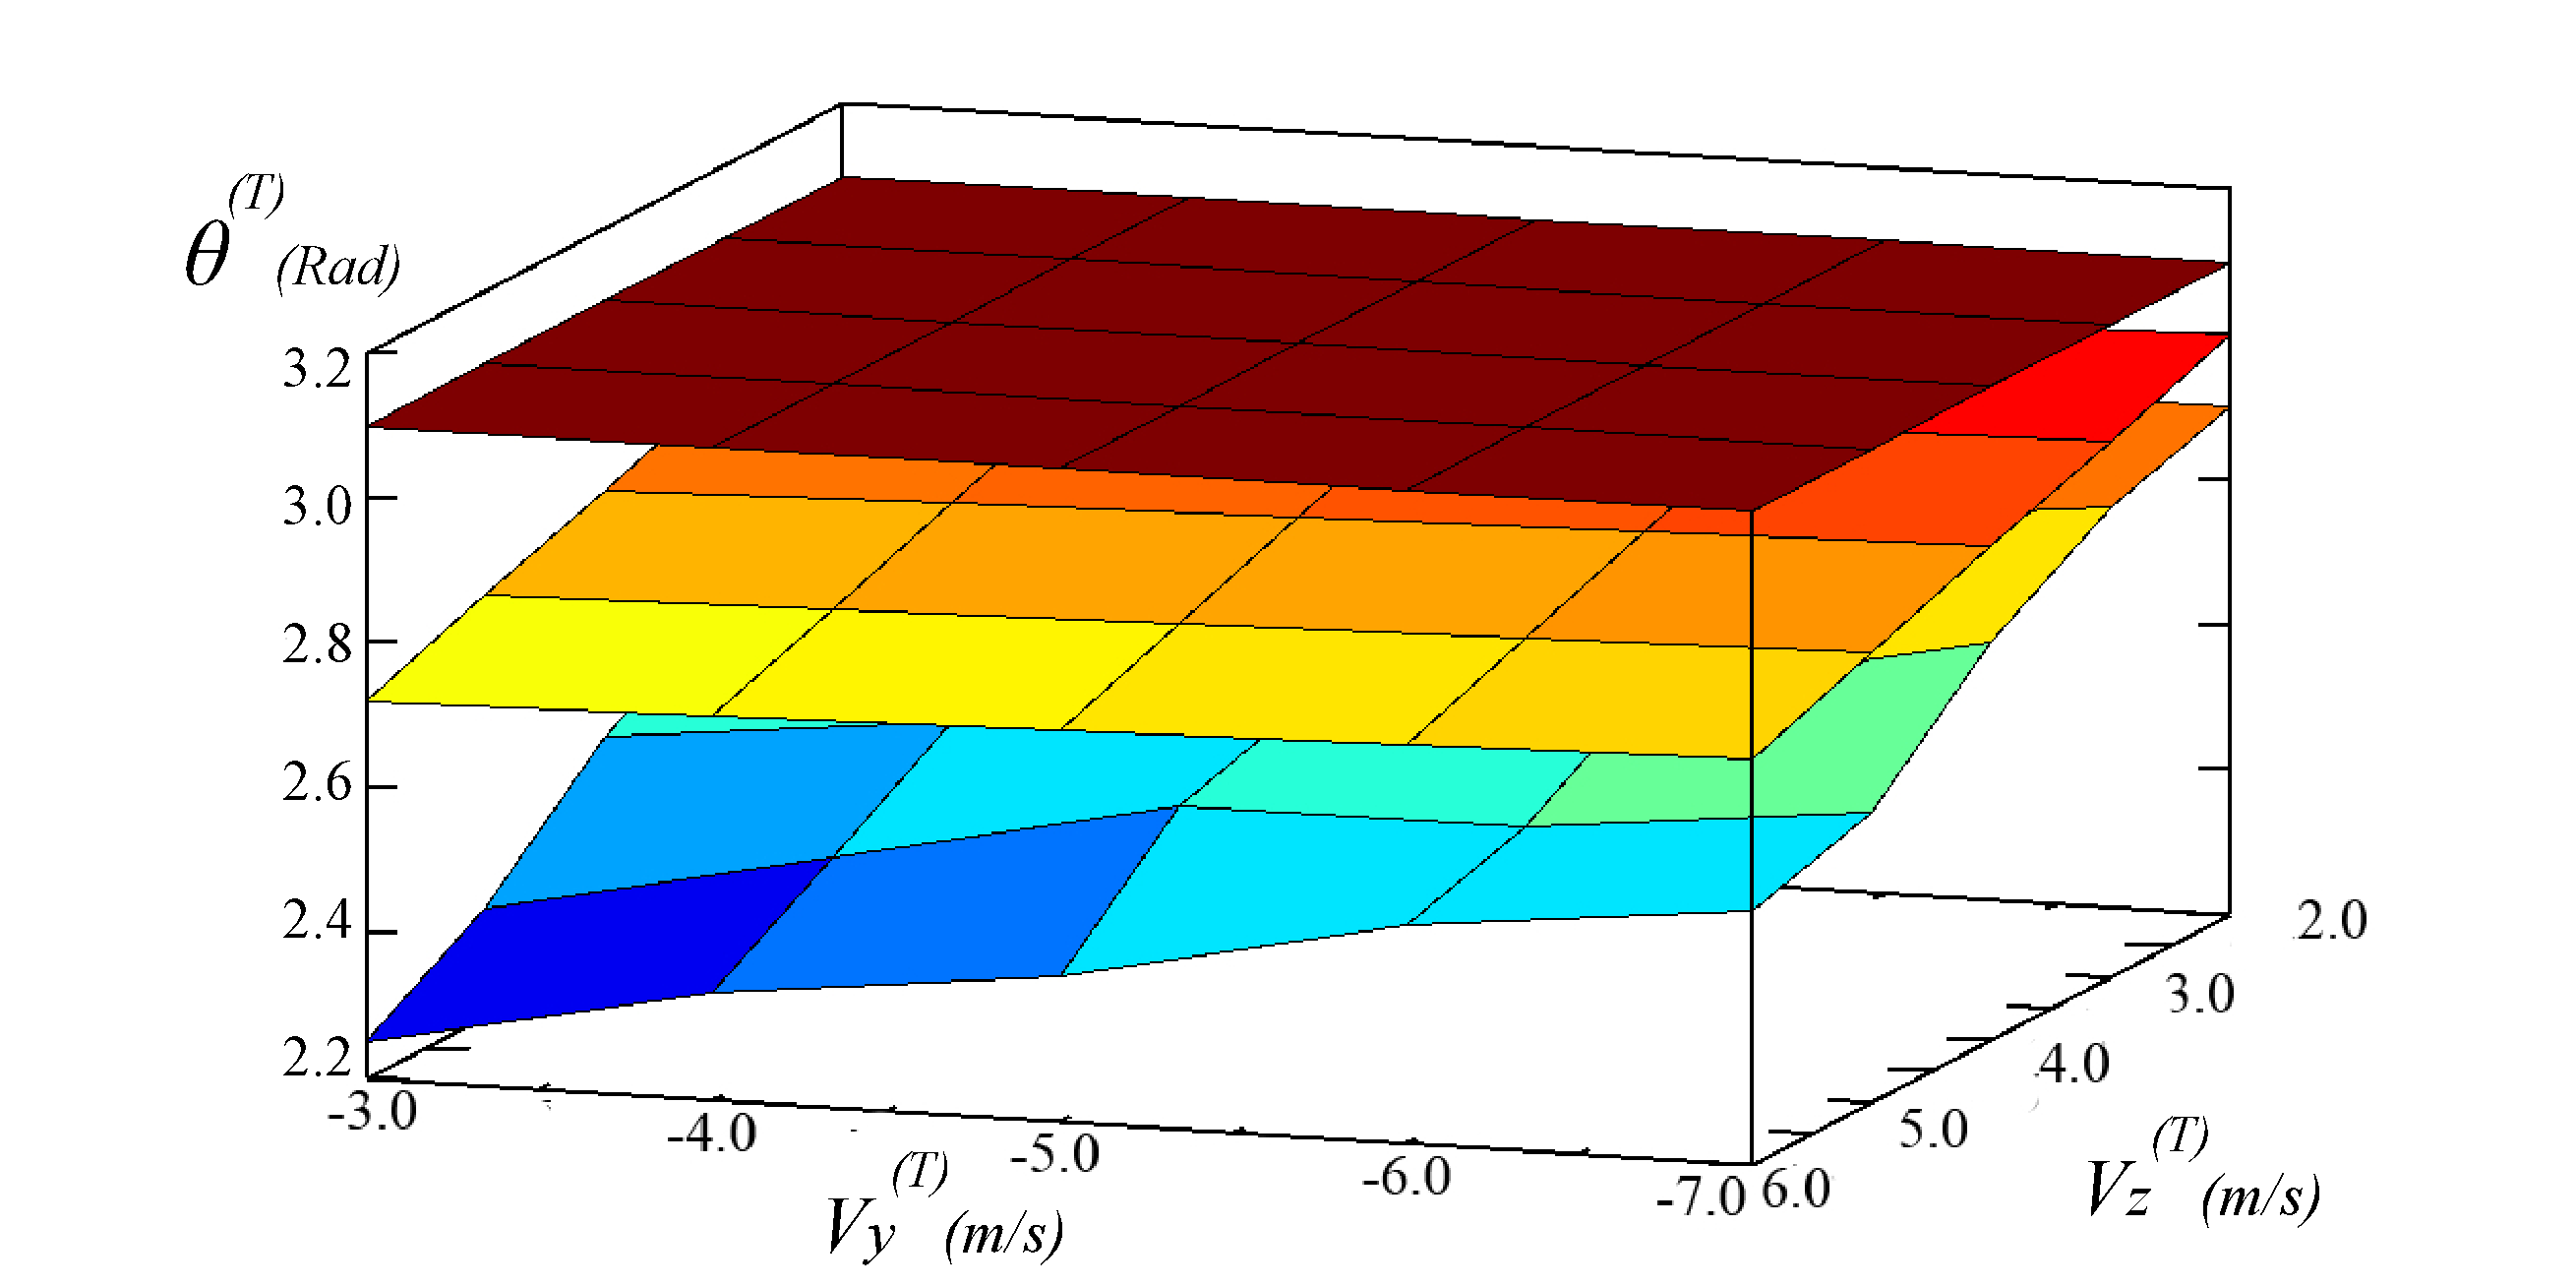
\includegraphics[width=0.49\textwidth]{images/sampleVYVZ}
  \caption{
    Samples for hands-first landing strategy. Successful samples are
    bounded between top and bottom planes along $\theta^{(T)}$
    axis. The middle plane, average of the two, indicates the linear
    relation of the ideal landing condition. 
  }
\ignorethis{
\emph{Top}: x-axis: 
    Domain spanned by $v_z^{(T)}$, $\omega_x^{(T)}$ and $\theta^{(T)}$ \emph{(Top)}
    Domain spanned by $v_z^{(T)}$, $v_y^{(T)}$ and $\theta^{(T)}$ \emph{(Bottom)}
  }
 \label{fig:landing_samplesPlanar}
\end{figure}
 
For the hands-first strategy with planar motion, we consider a
four-dimensional space spanned by $\theta^{(T)}$, $v_y^{(T)}$,
$v_z^{(T)}$ and $\omega_x^{(T)}$. Given a sample in the parameter
space, we run our landing controller to test whether the character can
successfully get up at the end. Empirical results from thousands of
random samples show that the successful region is mostly continuous
and linear (Figure \ref{fig:landing_samplesPlanar}). We can bound the
successful samples in the $\theta^{(T)}$ axis using two hyperplanes.
Taking the average of the maximum and the minimum planes, we derive a
linear relation between the angle of attack and the landing velocities as
\begin{equation}
\label{eqn:landing_approxLandingAngle}
\theta ^{(T)} = a \;v_y^{(T)} + b \;v_z^{(T)} + c \;\omega_x^{(T)} + d
\end{equation}
where $a$, $b$, $c$, and $d$ are the coefficients of the fitted
hyperplane. Note that Equation (\ref{eqn:landing_approxLandingAngle}) is a
sufficient but not necessary condition for successful landing. Most
points between the maximal and minimal hyperplanes also lead to
successful landing motions. This means that even when the character
cannot meet the landing condition exactly, it still has a good chance
to land successfully. For the feet-first strategy, in theory, we need
to consider all six dimensions of linear velocity and angular
velocity. However, our empirical results show that non-planar
velocities do not affect $\theta^{(T)}$ as long as they stay within a
reasonable bound (Figure \ref{fig:landing_sampleNonPlanar}). As a result, the
feet-first strategy is able to handle non-planner falling motion using
the same parameters (but different coefficients) in Equation
(\ref{eqn:landing_approxLandingAngle}).

\begin{figure}[ht]
\center
  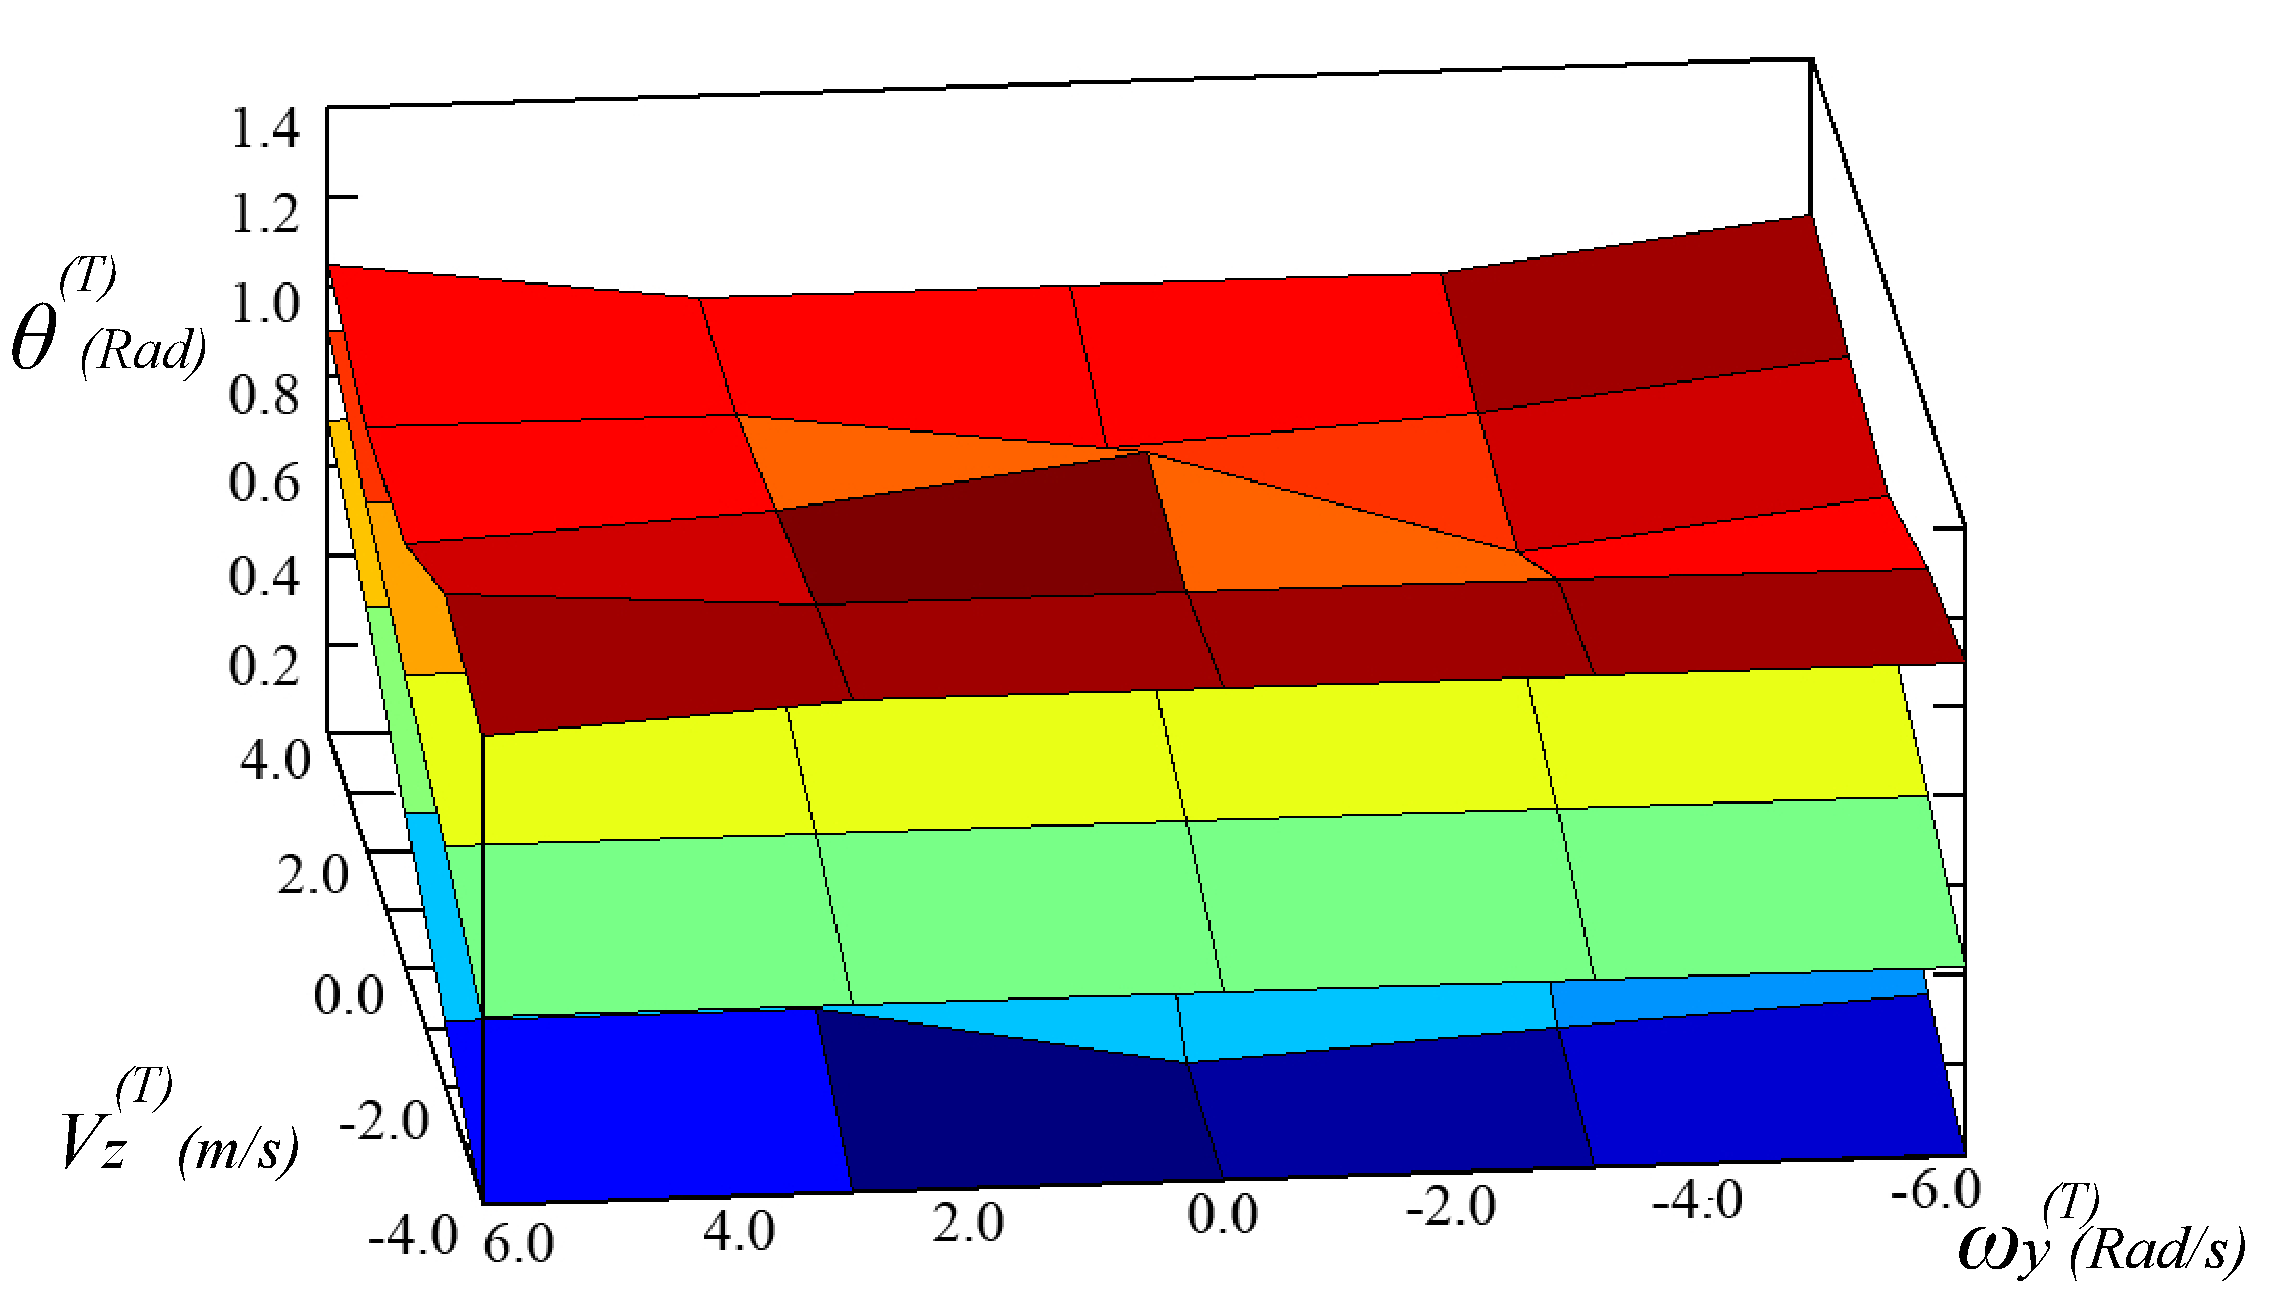
\includegraphics[width=0.51\textwidth]{images/sampleWYflat}
  \caption{
    Samples in the space of $v_z^{(T)}$, $\omega_y^{(T)}$, and
    $\theta^{(T)}$. The spinning velocity $\omega_y^{(T)}$
    has minimal effect on the success of a sample.
  }
 \label{fig:landing_sampleNonPlanar}
\end{figure}


\section{Airborne Phase}
Once the character decides on a landing strategy, the goal of the
airborne phase is to achieve the corresponding landing pose and
landing condition. Because momentum is conserved in air, the linear
velocity, the total airborne time $T$, as well as the angular momentum
are already determined by the initial condition of the fall.  However,
the character can still control the angular velocity $\omega_x^{(T)}$
and the angle of attack $\theta^{(T)}$ by varying its pose (\ie
actuated degrees of freedom (DOFs) excluding the global position and
orientation) to change the moment of inertia. To most effectively
achieve the desired landing condition, we design our airborne
algorithm based on the strategy employed in platform diving
competition, where a highly trained athlete performs a sequence of
predefined poses to manipulate the final orientation and angular
velocity.

To this end, our airborne controller uses a PD servo to track a
sequence of poses that lead to the ideal landing condition. 
The sequence of poses is replanned frequently to correct the errors
caused by perturbation and numerical approximation. Each time the
algorithm makes a new plan, an optimal sequence of poses from the
current moment to the landing moment is computed. This sequence
starts with the current pose $\vc{q}_0$ and ends at the desired
landing pose $\vc{q}_T$ (determined by the landing strategy), with a
duration of $T$ seconds. Our control algorithm searches for an
intermediate pose $\vc{q}^*$ and a duration $\Delta t^*$, such that
the character can reach the ideal landing condition by changing to
$\vc{q}^*$ immediately and holding the pose $\vc{q}^*$ for $\Delta
t^*$ seconds before changing to the final pose $\vc{q}_T$.

We formulate an optimization to solve for an intermediate pose $\vc{q}$
and its holding duration $\Delta t$ that can best achieve the ideal
landing condition. The cost function  $g(\vc{q}, \Delta t)$ is defined
in Equation \ref{eqn:landing_landingCondition}.

\begin{equation}
g(\vc{q}, \Delta t) = \theta^{(T)}(\vc{q}, \Delta t) - a \;v_y^{(T)} - b \;v_z^{(T)} - c\;
\omega_x^{(T)}(\theta^{(T)}) - d
\label{eqn:landing_landingCondition}
\end{equation}
Note that $\omega_x^{(T)}$ is a function of $\theta^{(T)}$ because we
need global orientation of the character at time $T$ to compute the
global angular velocity. If we can compute $\theta^{(T)}$, Equation
(\ref{eqn:landing_landingCondition}) can be readily evaluated. Unfortunately,
for a complex 3D multibody system, an analytical solution for
$\theta^{(T)}$ is not available. We could resort to numerical
simulation of the entire airborne phase, in which the character goes
through $\vc{q}_0$, $\vc{q}^*$, and $\vc{q}_T$ subsequently. However,
involving forward simulation of a full skeleton in the cost function
is too costly for our real-time application.\ignorethis{However, we
  cannot compute $\theta^{(T)}$ analytically and have to resort to
  numerical simulation of the entire airborne phase, in which the
  character goes through $\vc{q}_0$, $\vc{q}$, and $\vc{q}^T$
  subsequently. Such simulation of a full skeleton is too costly for a
  real-time application.} Instead, we simulate a simple proxy model
with only six DOFs. When the character is holding a pose, the proxy
model behaves like a rigid body with a fixed inertia.  When the
character transitions from one pose to another, we assume the inertia
of the proxy model changes linearly within a fixed duration $\Delta
t_C$ ($\Delta t_C = 0.1s$ in our implementation). By simulating the proxy
model for the duration of $T$, we obtain the angle of attack
$\theta^{(T)}$ and angular velocity $\omega^{(T)}$ as
follows.
\begin{eqnarray}
\vc{R}(\theta^{(T)}) = \vc{R}(\theta^{(0)}) + \int_{t=0}^{\Delta t_c}
[\vc{I}^{-1}_{A}(t)\vc{L}]\vc{R}(\theta^{(t)}) dt \nonumber \\ 
+ \int_{t=\Delta t_c}^{\Delta t_c + \Delta
  t}[\vc{I}^{-1}(\vc{q},\theta^{(t)})\vc{L}]\vc{R}(\theta^{(t)}) dt \nonumber \\ + \int_{t=\Delta
  t_c+\Delta t}^{2 \Delta t_c + \Delta t}
[\vc{I}^{-1}_{B}(t)\vc{L}]\vc{R}(\theta^{(t)}) dt \nonumber \\ +
\int_{t=2 \Delta t_c+\Delta t}^T
[\vc{I}^{-1}(\vc{q}_T,\theta^{(t)})\vc{L}]\vc{R}(\theta^{(t)}) dt; \\
\omega^{(T)} = \vc{I}^{-1}(\vc{q}_T,\theta^{(T)})\vc{L}
\end{eqnarray}
where $\vc{R}$ is the rotation matrix, $\vc{I}(\vc{q})$ is an inertia
matrix evaluated at pose $\vc{q}$, and $\vc{L}$ is the angular
momentum. $\vc{I}_{A}(t)$ is an interpolated inertia matrix between $\vc{I}(\vc{q}_0)$ and
$\vc{I}(\vc{q})$, and similarly, $\vc{I}_{B}(t)$ is an interpolated matrix between
$\vc{I}(\vc{q})$ and $\vc{I}(\vc{q}_T)$. The operator $[\;]$ represents the skew
symmetric matrix form of a vector.

% \ignorethis{
% an airborne character can
% only control its pose (\ie actuated degrees of freedom) to change
% the moment of inertia, but cannot directly control the global position and orientation. To this end, we design an airborne controller that
% determines a sequence of poses and uses proportional-derivative (PD)
% servos to track them. In our problem, the initial pose $\vc{q}_0$ is
% determined by the initial conditions of the fall, and the final pose
% $\vc{q}_T$ is determined by the landing strategy. Our algorithm,
% therefore, searches for an intermediate pose $\vc{q}^*$ from a
% predefined pose set and a duration $\Delta t^*$ such that the
% character can achieve the ideal landing condition by changing from
% $\vc{q}_0$ to $\vc{q}^*$ immediately after the fall begins, holding
% $\vc{q}^*$ for $\Delta t^*$ seconds, and changing to $\vc{q}_T$ until
% the end of airborne phase.

% To search for the optimal control parameters, $\vc{q}^*$ and $\Delta
% t^*$, we need to define a cost function, $g(\vc{q}, \Delta t)$ which
% evaluates how well the falling motion achieves the ideal landing
% condition for a given estimate of control parameters. We will first
% describe how we derive landing conditions, followed by the details of
% the search algorithm.


% \paragraph{Search for optimal control parameters.}
% Using the derived landing condition, we now define the cost function
% as

% \begin{equation}
% g(\vc{q}, \Delta t) = \theta^{(T)}(\vc{q}, \Delta t) - a \;v_y^{(T)} - b \;v_z^{(T)} - c\;
% \omega_x^{(T)} - d
% \label{eqn:landingCondition}
% \end{equation}

% Due to conservation of momentum and a known final pose, $v_y^{(T)}$,
% $v_z^{(T)}$ and $\omega_x^{(T)}$ can be computed from the initial
% condition of the fall. The only unknown value in Equation
% \ref{eqn:landingCondition} is $\theta^{(T)}$, which depends on the
% control parameters, $\vc{q}$ and $\Delta t$. Because we cannot compute
% $\theta^{(T)}$ analytically, we propose to simulate the entire
% airborne motion, going through the initial pose $\vc{q}_0$, the
% estimated intermediate pose $\vc{q}$, and the final pose $\vc{q}_T$,
% subsequently.

% However, simulating a full skeleton is too costly for efficient
% evaluation of $g(\vc{q}, \Delta t)$. Instead, we simulate a simple
% model with only six DOFs as a rigid body, but we allow its inertia to
% vary over time. When the character transitions from one pose to
% another, we assume the inertia changes gradually within a fixed
% duration $\Delta t_C$. The angle of attack for the simple model can be
% expressed as following equation and integrated numerically:
% \begin{eqnarray}
% \vc{R}(\theta^{(T)}) = \vc{R}(\theta^{(0)}) + \int_{t=0}^{\Delta t_c}
% [\vc{I}^{-1}(\vc{q}_A(t))\vc{L}]\vc{R}(\theta^{(t)}) \nonumber \\ 
% + \int_{t=\Delta t_c}^{\Delta t_c + \Delta
%   t}[\vc{I}^{-1}(\vc{q})\vc{L}]\vc{R}(\theta^{(t)}) \nonumber \\ + \int_{t=\Delta
%   t_c+\Delta t}^{2 \Delta t_c + \Delta t}
% [\vc{I}^{-1}(\vc{q}_B(t))\vc{L}]\vc{R}(\theta^{(t)}) \nonumber \\ +
% \int_{t=2 \Delta t_c+\Delta t}^T [\vc{I}^{-1}(\vc{q}_T)\vc{L}]\vc{R}(\theta^{(t)})
% \end{eqnarray}
% where $\vc{R}$ is the rotation matrix, $\vc{I}(\vc{q})$ is an inertia
% matrix evaluated at pose $\vc{q}$, and $\vc{L}$ is the angular
% momentum. $\vc{q}_A(t)$ is an interpolated pose between $\vc{q}_0$ and
% $\vc{q}$, and similarly, $\vc{q}_B(t)$ is an interpolated pose between
% $\vc{q}$ and $\vc{q}_T$. The operator $[\vc{a}]$ is the skew symmetric
% matrix of a vector $\vc{a}$.
% }
% \ignorethis{
% To interpolate the inertia, inertia matrices are decomposed into a rotation matrix
%  $\mat{R}$ and a axis-aligned matrix $\mat{I_A}$ using Singular Value Decomposition 
% and interpolated using slerp and weighted sum. 

% \begin{eqnarray}
% \mat{I_0} = \mat{R_0} \mat{I}_{A0} \mat{R_0}^T \nonumber \\
% \mat{I_1} = \mat{R_1} \mat{I}_{A1} \mat{R_1}^T \nonumber \\
% \mat{R}(w) = slerp(\mat{R_0}, \mat{R_1}, w) \nonumber \\
% \mat{I}(w) = \mat{R}(w) (w \mat{I}_{A0} + (1-w)\mat{I}_{A1}) \mat{R}(w)^T \nonumber
% \end{eqnarray}

% While inertia is updated, angular velocity should be updated as well
% to preserve angular momentum. A rigid body simulation is relatively
% inaccurate comparing to the full simulation, but it is enough to
% approximate the landing angle $\theta(T)$ as shown in Figure
% \ref{fig:inertiaTrajectory}. After the simulaton ended, the cost
% functions returns the difference between the current orientation and
% the desired landing angle of attack $\theta(T)$.  
% }

% %% \sehoon{
To formulate an efficient optimization for real-time application, we
represent the domain of intermediate pose as a finite set of candidate
poses, instead of a continuous high-dimensional Euclidean space. This
simplification is justified because a handful of poses is sufficient
to effectively change the moment of inertia of the character. As a
preprocess step, our algorithm automatically selects the candidate set
$\mat{Q}$ from a motion capture sequence in which the subject performs
range-of-motion exercise. The selection procedure begins with a seed
pose $\bar{\vc{q}}_0$ and increments the set by adding a new pose
$\bar{\vc{q}}_{new}$ which maximizes the diversity of inertia
(Equation \ref{eqn:landing_selectingCandidate}). In our experiment, 16 poses
are sufficient to present a variety of moment of inertia
(Figure \ref{fig:landing_candidatePoses}).



% \ignorethis{ The intermediate pose is chosen from a set of predefined
%   poses $\mat{Q}=\{\vc{q}^*_0, \vc{q}^*_1, ... \}$ that can most
%   effectively change each of the six values of the full-body inertia
%   (Figure \ref{fig:candidatePoses}).  We select the set $\mat{Q}$
%   automatically from the captured range of motion.  We start from a
%   selected seed pose $\vc{q}^*_0$ and increment the set by adding a
%   new pose $q^*_{new}$ which maximizes the diversity of inertia
%   (Equation \ref{eqn:selectingCandidate}).  In our experiment, 16
%   poses are compact but sufficient to handle a wide range of initial
%   conditions.}
% %% }

\begin{equation}
\label{eqn:landing_selectingCandidate}
\bar{\vc{q}}_{new} = \argmax_{\vc{q} \in M} (\min_{\bar{\vc{q}}_j \in Q} \| I(\vc{q}) - I(\bar{\vc{q}}_j)\|) \}
\end{equation}
where $M$ contains the poses in the range-of-motion sequence, $Q$
contains the currently selected candidate poses, and $I(\vc{q})$
computes the inertia of pose $\vc{q}$.

%% During the optimization, we loop over each candidate pose in $Q$. For
To find optimal $\vc{q}^*$ and $\Delta t^*$ for each plan, we start from the current pose as $\vc{q}_0$ and loop over each candidate pose in $Q$. For
each candidate pose $\bar{\vc{q}}_i$, we search for the best $\Delta
t$ such that $g(\bar{\vc{q}}_i, \Delta t)$ is minimized. The search can
be done efficiently using one-dimensional Fibonacci algorithm and the
proxy-model simulation. The optimal intermediate pose $\vc{q}^*$ and
its optimal duration $\Delta t^*$ are used for airborne control.

\begin{figure}[ht]
\center
  %% \includegraphics[width=3.2in]{images/AirbornePoses}
  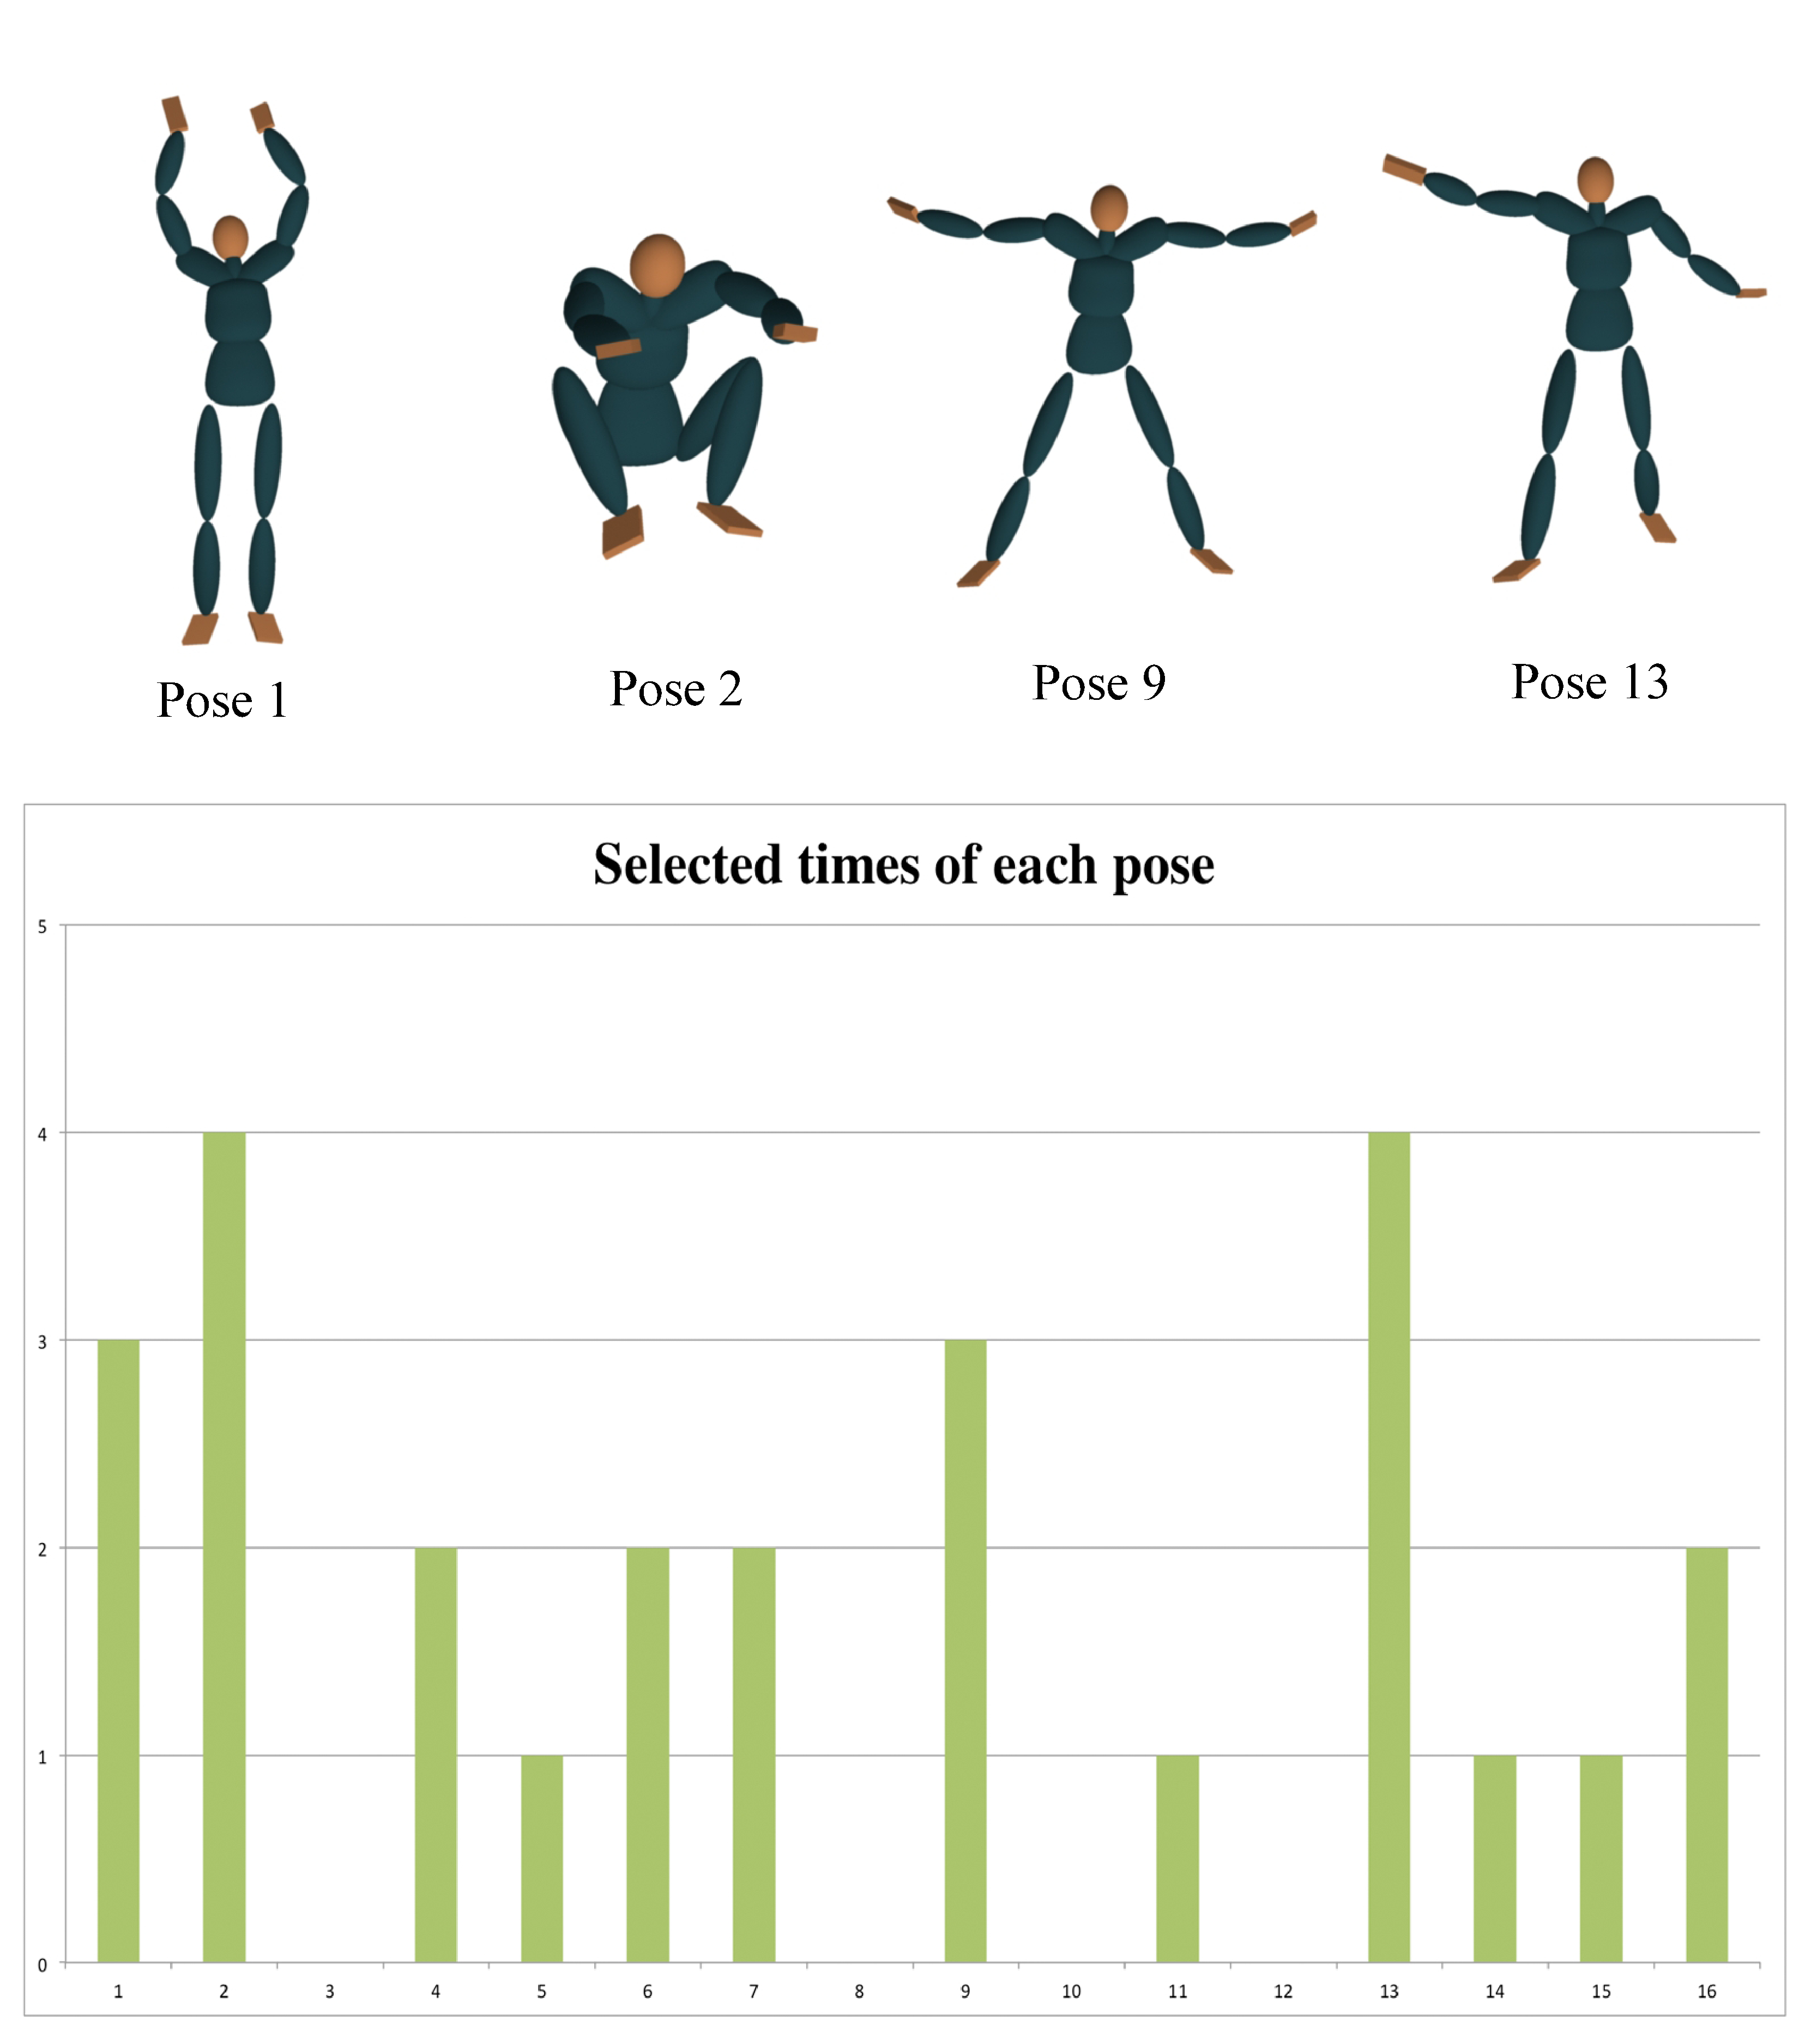
\includegraphics[width=4.2in]{images/PoseWithStats}
  %% \caption{A few popular candidate poses from $\mat{Q}$.
  \caption{
    Among 16 poses in $\mat{Q}$, pose 1, 2, 9, and 13 are frequently 
    selected by the airborne controller
  }
 \label{fig:landing_candidatePoses}
\end{figure}

By design, our algorithm trades off accuracy for efficiency; we use a
fast but less accurate proxy-model simulation and a small set of
predefined poses. Our algorithm is very efficient so that the
character can frequently reassess the situation and replan new poses
to correct any errors or adapt to unexpected perturbations. 

The frequency of replanning can be determined differently for
$\vc{q}^*$ and $\Delta t^*$. In our implementation, we replan
$\vc{q}^*$ at a much lower frequency than $\Delta t^*$ to avoid
unnatural frequent change of poses. In addition, we stop replanning
when the character is within $0.3$ seconds away from the ground.

\section{Landing Phase}
\label{sec:landing_landing}
During landing, the character braces for impact, executes rolling
action, and gets up on its feet. Although these three stages take very
different actions, they share common control goals: modulating the COM
and posing important joints.  We apply the same control mechanism via
\emph{virtual forces} and \emph{PID joint-tracking} to produce the
final control forces for the forward simulator (Figure
\ref{fig:landing_landingOverview}).

\begin{figure}[htbp]
\center
  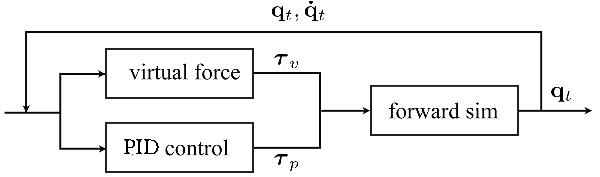
\includegraphics[width=3.2in]{images/landingOverview}
  \caption{Landing phase controller.}
 \label{fig:landing_landingOverview}
\end{figure}

Virtual forces are effective in controlling the motion of the COM. To
achieve a desired acceleration of the COM, $\ddot{\vc{c}}$, we compute
the virtual force as $\vc{f}_v = m \ddot{\vc{c}}$ where $m$ is the mass of the
character. The equivalent joint torque as if applying $\vc{f}_v$ to a
point $\vc{p}$ on the body is $\tau_v = \vc{J}^T (\vc{p}) \vc{f}_v$,
where $\vc{J}(\vc{p})$ is the Jacobian computed at the body point
$\vc{p}$.
If $\vc{p}$ is on a body node in contact with the ground, 
we apply the opposite force ($\vc{f}_v = -m \ddot{\vc{c}}$) in order to
generate a ground reaction force that pushes the COM in the desired direction.
To prevent the character from using excessively large joint
torques, we limit the magnitude of the sum of virtual forces.  A
successful landing motion also requires posing a few important joints
at each of the three stages. We track these partial poses with PID
servos: $\tau_p = k_p (\bar{q} - q) + k_i \int (\bar{q}_t - q_t) dt -
k_v \dot{q}$, where $k_p$, $k_i$ and $k_v$ are the proportional,
integral, and derivative gains respectively, and $\bar{q}$ is the
desired joint angle.  The final control torque is $\tau_v+\tau_p$.
We limit the magnitude of the virtual force to $3000N$ to prevent
excessive usage of joint torques.



\subsection{Impact Stage}
\label{sec:landing_impact}


Impact stage is the most critical stage during landing, which requires
careful control and execution. Human athletes tend to act like a
spring to absorb the effect of impact by flexing their joints between
the points of first contact and the COM. Meanwhile, they also utilize
friction force from the ground contact to adjust forward linear
momentum and angular momentum. Applying these principles, our
algorithm utilizes virtual force technique to achieve contact forces
for desired momentum. In addition, we use joint tracking to provide
sufficient stiffness at contacting limbs and smooth transition to the
next stage. If the character chooses the hands-first strategy, the
final pose at the end of compression can seamlessly connect to the
rolling stage. With the feet-first strategy, an additional
``thrusting'' step is required to transition to the rolling stage. We
define a ``ready-to-roll'' pose that guides the character toward a
rolling motion (Figure \ref{fig:landing_landingPoses}, Right). During this additional
step, the character tracks the ready-to-roll pose while using its feet
to thrust forward after its COM compressed to the lowest point (Figure
\ref{fig:landing_feet-first}).

\begin{figure}[htbp]
\center
%% \begin{minipage}{0.35\textwidth}
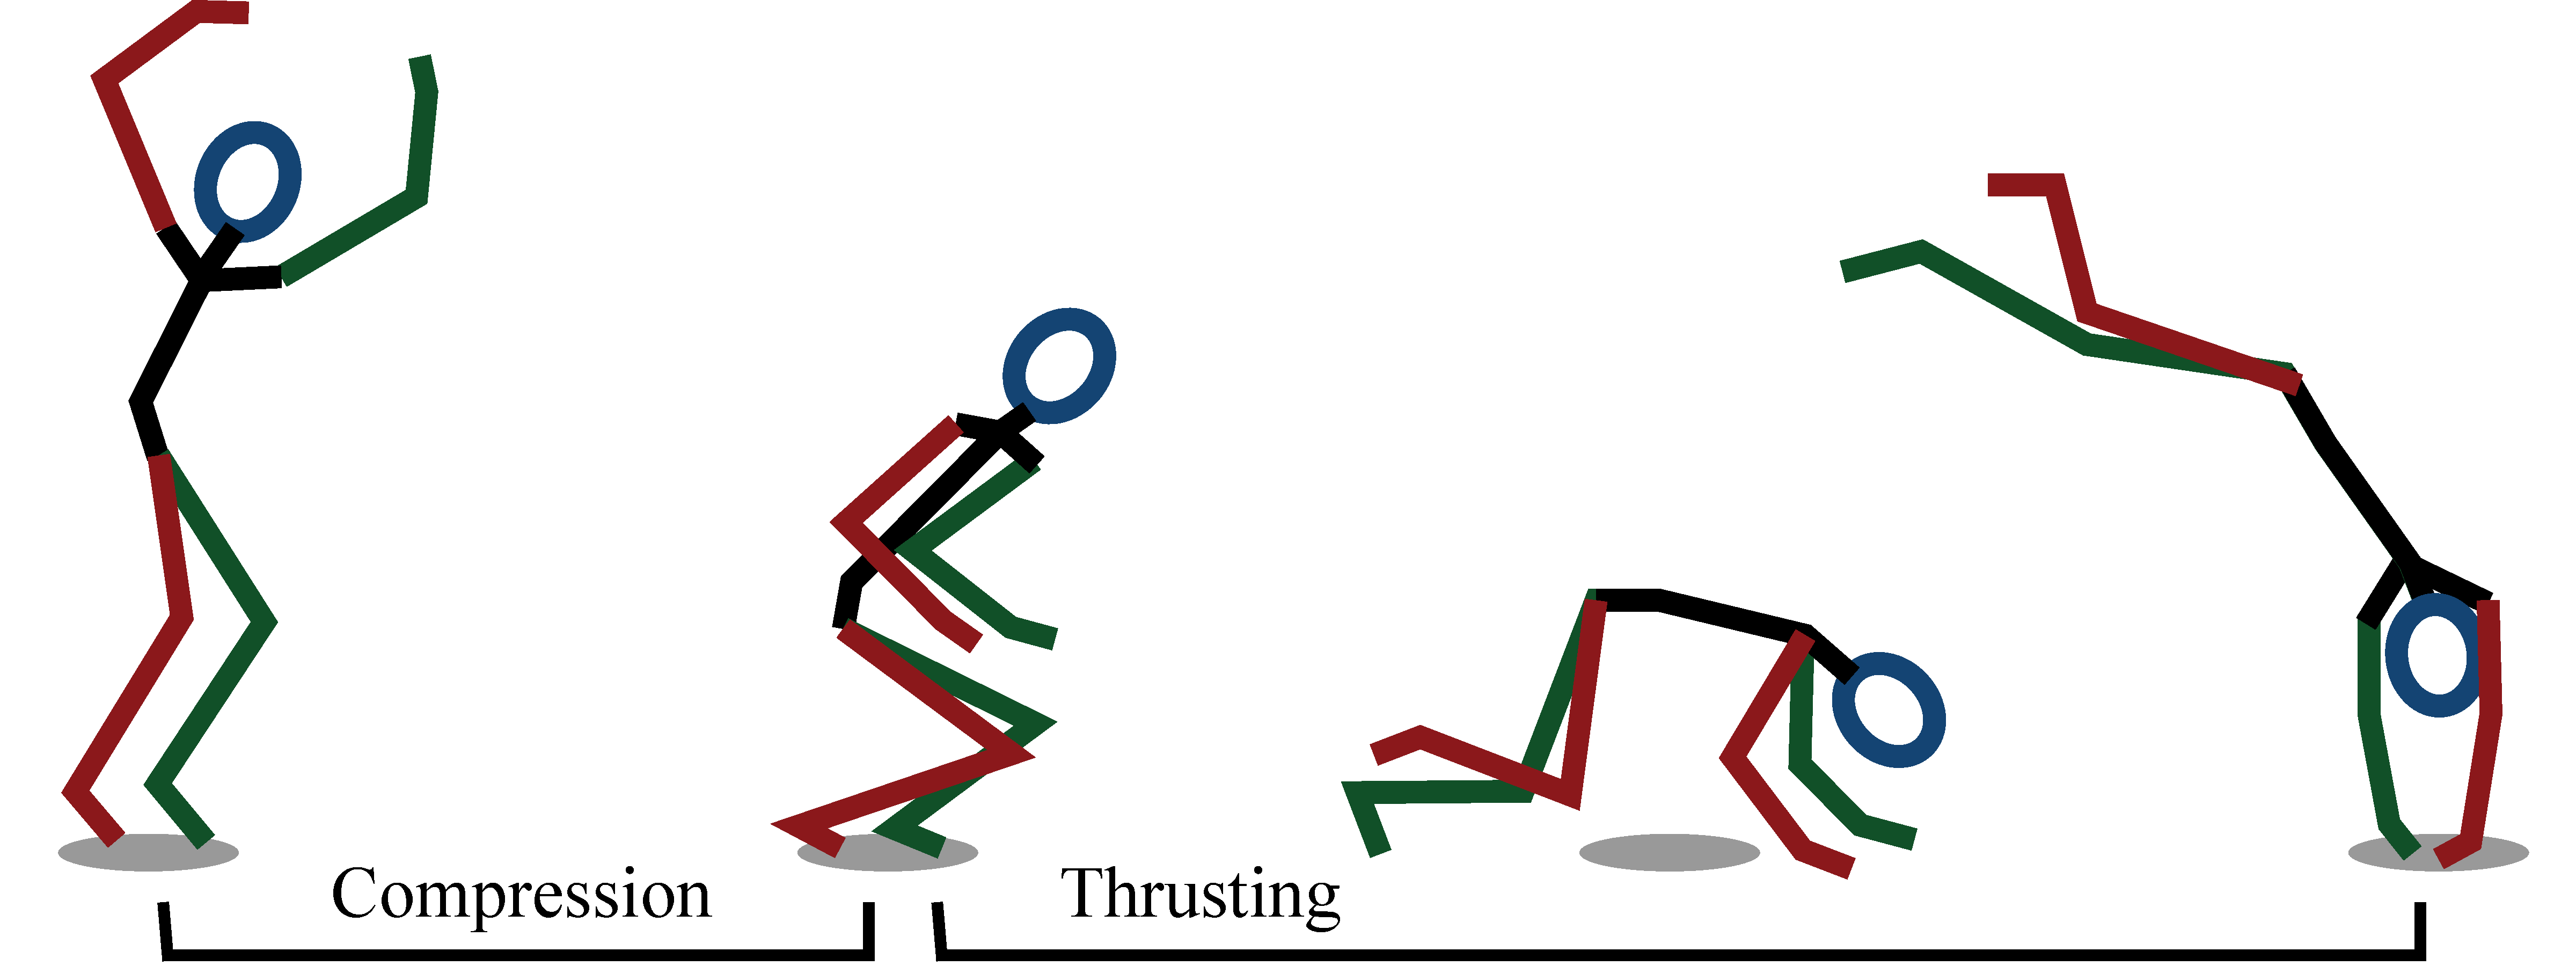
\includegraphics[width=4.2in]{images/feet-first}
\caption{Two-step impact stage for the feet-first strategy.}
\label{fig:landing_feet-first}
%% \end{minipage}
%% \begin{minipage}{0.1\textwidth}
%% 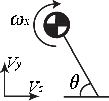
\includegraphics[width=0.8in]{images/COM}
%% \caption{}
%% \label{fig:COM}
%% \end{minipage}
\end{figure}
\ignorethis{
Our algorithm has two different landing styles for impact stage: 
\emph{Landing with hands} and \emph{Landing with feet}. They are not 
only different in the body parts for the first contact but also 
different in the strategies to control the trajectory of COM. While
\emph{Landing with hands} tries to achieve the desired forward momentum
at the lowest point of the COM, \emph{Landing with feet} divides the task
into two stages: compression and thrust. At the compression stages, 
the character acts like a damped spring to absorb all the velocities 
except the forward direction by crouching itself. When the COM reaches 
the bottom point, the algorithm enters the thrust stage and 
commands the character to kick the ground for the desired forward 
linear and angular momentum.}

\textbf{Virtual force.} The most important goal during the impact
stage is to stop the downward momentum before the character tragically
crashes into the ground. We do so by applying virtual forces to
control the vertical position and velocity of the COM. In addition,
our algorithm favors virtual forces that result in temporally smooth
ground reaction forces to distribute the impact evenly over
time. \ignorethis{in hopes of avoiding large joint stress at all
  times.} With these control goals, our algorithm aims to
use constant acceleration of the COM to achieve the desired COM
position $\bar{c}_y$ and velocity $\bar{\dot{c}}_y$ from the current
state ($c_y$ and $\dot{c}_y$).
\begin{equation}
\label{eqn:landing_controlY}
\ddot{c}_y = \frac{1}{2}(\bar{\dot{c}}_y^2 - \dot{c}_y^2) / (\bar{c}_y-c_y)
\end{equation}
A virtual force of $-m\ddot{c}_y$ in the vertical direction is then evenly
distributed to the end-effectors that are in contact with the ground.

Virtual forces in the horizontal direction are important to achieve
the desired forward linear momentum and angular momentum at the end of 
compression, or to achieve the desired forward thrust for the feet-first
strategy. We use a simple feedback mechanism to compute the desired
horizontal acceleration of the COM.
\begin{equation}
\label{eqn:landing_controlXZ}
\ddot{c}_{x/z} = k_v (\bar{\dot{c}}_{x/z} - \dot{c}_{x/z})
\end{equation}
where $\bar{\dot{c}}_{x/z}$ is the desired COM velocity in forward and
lateral directions and $k_v$ is the damping coefficient. The
corresponding virtual force is distributed to the contacting
end-effectors inversely proportional to their distances to the
COM.

\begin{table}
\center
{
%% \small
\caption{Control parameters. 
}


\begin{tabular}{|c |c|c|c|c|c| }
\hline
\label{tab:landing_tracking}

& {\small Hip} & {\small Lower spine } & {\small Upper spine } & {\small Neck } & {\small Knee } \\ \hline 
\textbf{$k_p$} & {\small 90.0} & {\small 300.0}& {\small 180.0}& {\small 10.0} & {\small 60.0} \\ \hline 
\textbf{$k_d$} & {\small 20.0} & {\small 60.0} & {\small 40.0} & {\small  2.0} & {\small 13.0} \\ \hline


& {\small Ankle } & {\small Clavicle } & {\small Shoulder} & {\small Elbow } & {\small Wrist } \\ \hline 
\textbf{$k_p$} & {\small 15.0} & {\small 180.0}& {\small 120.0}& {\small 60.0} & {\small  9.0} \\ \hline
\textbf{$k_d$} & {\small  6.0} & {\small 40.0} & {\small 27.0} & {\small 13.5} & {\small  4.0} \\ \hline

%% \textbf{$k_p$} 
%% & {\tiny 90.0} & {\tiny 300.0}& {\tiny 180.0}& {\tiny 10.0} & {\tiny 60.0} 
%% & {\tiny 15.0} & {\tiny 180.0}& {\tiny 120.0}& {\tiny 60.0} & {\tiny  9.0} \\ \hline

%% \textbf{$k_d$} 
%% & {\tiny 20.0} & {\tiny 60.0} & {\tiny 40.0} & {\tiny  2.0} & {\tiny 13.0} 
%% & {\tiny  6.0} & {\tiny 40.0} & {\tiny 27.0} & {\tiny 13.5} & {\tiny  4.0} \\ \hline
%% \end{tabular}

%% \begin{tabular}{|c|c|c|c|c|c|}
\hline
{\small \textbf{$\bar{c}_y$} } &
{\small \textbf{$\bar{\dot{c}}_y$} } &
{\small \textbf{$\bar{\dot{c}}_{x/z}$} } &
{\small \textbf{$k_v$} } &
{\small \textbf{$k_p$} (Eq \ref{eqn:landing_controlRoll}) } &  
{\small \textbf{$\omega_{MAX}$} } \\ \hline

{\small 0.4m} & {\small 0.0m/s} & {\small 4.0m/s} & {\small 500} & {\small 800} & {\small 3.3 Rad/s} \\ \hline
\end{tabular}
}
\end{table}


\textbf{Joint tracking.} In addition to virtual forces, we use PID
servos to maintain joint angles of the torso and limbs that are not in
contact, while limbs in contact with the ground act like viscous
dampers (PID control with a zero spring coefficient). We also use PID
control to keep the chin tucked to reduce the chance of the head
impacting the ground. Please see Table \ref{tab:landing_tracking} for all the
parameters in our implementation. We set the constant integral gain
$k_i$ of contacting limbs as $50$, and $0$ for all other joints.



\subsection{Rolling Stage}
\label{sec:landing_rolling}
Once the character's COM passes the hand-ground contact area with
sufficient forward linear and angular momentum, rolling becomes a
relatively easy task. As long as the character is holding a pose with
a flexed torso, a reasonable rolling motion will readily carry out. If
the character wishes to land back on its feet and get up after
rolling, it must also maintain forward momentum and lateral balance
during the roll.

\textbf{Virtual force.} To this end, we apply a virtual force to guide
the horizontal position of the COM toward the feet area, while
restricting it above the support polygon formed by contact points. The
virtual force is applied on the character's hands so that it can use
the entire upper body to maintain momentum and
balance. The virtual force produces the desired acceleration of the COM 
computed using a feedback mechanism:
\begin{equation}
\label{eqn:landing_controlRoll}
\ddot{c}_{x/z} = k_p (\bar{c}_{x/z} - c_{x/z})
\end{equation}
where the desired position $\bar{c}$ is set to be the location of the
left foot.

\textbf{Joint tracking.} During rolling, the character tracks a simple
pose to tuck the head, flex the torso, and position the legs
appropriately. We treat legs asymmetrically to both facilitate
momentum control and improve the aesthetics of the motion. When the
character rolls on its back, it brings the left knee closer to the
chest and casually stretches the right leg. This arrangement helps the
character to regulate the angular velocity using the right leg while
getting ready to stand up on its left foot. Based on the forward
angular velocity at the beginning of the rolling stage, we adjust the
desired tracking angles for the right knee as:
\begin{equation}
\label{eqn:landing_controlLeg}
\theta_R = max( (1 - \omega_x / \omega_{MAX}) \pi, 0 )
\end{equation}
\ignorethis{
Our algorithm applies PD control on head,
torso and legs to track some desired joint angles. Head and torso are
bended in forward direction to make the back of the character round
for smooth rolling.  For controlling legs, we assign the different
tasks to left and right legs.  The left leg is always tightly tucked
toward torso and prepared for stand up.  On the other hand, the right
leg is relatively more stretched to regulate the inertia based on the
current angular velocity. For instance, the right leg is tightly
tucked in low speed and fully straightened in the opposite case. The
role of left and right legs can be swapped.
}
\subsection{Getting-Up Stage}
The last stage of landing phase is to stand up using the remaining
forward momentum. When the COM passes the foot contact, the character
will start to elevate its COM to a desired height.

\textbf{Virtual force.} Similar to previous stages, we again apply
virtual forces on the feet and the hands to control the vertical and
the horizontal positions of the COM respectively. We compute $\ddot{c}_y$
using the same formula from \secref{landing_impact} with different desired
height of the COM. For $\ddot{c}_{x/z}$, we use the same formula as
in \secref{landing_rolling}.

\textbf{Joint tracking.} During the getting-up stage, our algorithm
simply tracks the torso and the head to straighten the spine and untuck the chin.

\ignorethis{
\section{Landing Planner}
\label{sec:landingplanner}

\begin{figure}[ht]
\center
  \includegraphics[width=3.2in]{images/abstractmodel}
  \caption{Abstract Model for Landing Motion}
 \label{fig:landing_abstractmodel}
\end{figure}

The goal of landing planner is to guide COM for a smooth transition between 
airborne planner and rolling planner.
To illustrate the character at landing, we construct an abstract model which is 
a single point mass connected to the fixed contact point (Figure \ref{fig:landing_abstractmodel}).
In other words, it is similar to the inverted pendulum model with the varying length rod. 
To prepare rolling, we want to regulate the linear and angular velocity 
when the point mass is vertical to the contact point ($t = T_v$).
Since there are an infinite number of solutions, we assume 
the constant contact force $\vc{\bar{F}}_C$ to distribute the impact over time.

Therefore, our problem is finding the optimal landing orientation $\mat{R}_L$ 
and duration $T_v$ to achieve the desired linear and angular velocity, 
$\bar{\vc{v}}_{v}$ and $\bar{\vc{\omega}}_{v}$.
From the given $\mat{R}_L$ and the length between COM and the desired end-effectors $l_0$, 
we can calculate the position of COM at the landing $\vc{C}(0)$.
In the similar manner, we can obtain $\vc{C}(T_v)$ from the desired key-frame pose.
With the initial and final positions of COM, we can calculate the desired 
contact force $\vc{\bar{F}_C}$ by solving the following equation:

\begin{equation}
\label{eqn:landing_landingcom}
\vc{C}(T_V) = \vc{C}(0) + \vc{v}(0) T_v + \frac{\vc{\bar{F}}_C}{2m}T_v^2
\end{equation}

In fact, equation \ref{eqn:landing_landingcom} gives us the complete trajectory of COM.
Based on this, we can calculate the linear and angular velocity at time $T_v$.

\begin{eqnarray}
\vc{L}(T_v) = \vc{L}(0) + \int^{T_v}_{0} \vc{C}(t) \times \vc{\bar{F}}_C dt \\
\vc{v}(T_v) = \vc{v}(0) + \frac{\vc{\bar{F}}_C}{m}T_v \\
\vc{\omega}(T_v) = \mat{I}(T_v)^{-1} L(T_v)
\end{eqnarray}

We formulate the optimization for $\mat{R}_L$ and $T_v$
to minimize the difference between the velocity at $T_v$ and the desired velocity.

\begin{equation}
(\mat{R}_L^*, T_v^*) = \argmin_{\mat{R}_L, T_v} 
(w_0|\vc{v}(T_v) - \bar{\vc{v}}_{v}| + w_1|\vc{\omega}(T_v) - \bar{\vc{\omega}}_{v}|)
\end{equation}

Since the optimization problem is non-linear and non-differentiable, 
we apply a derivative free optimization algorithm to solve.
}

\section{Results}

\begin{figure}[ht]
\center
  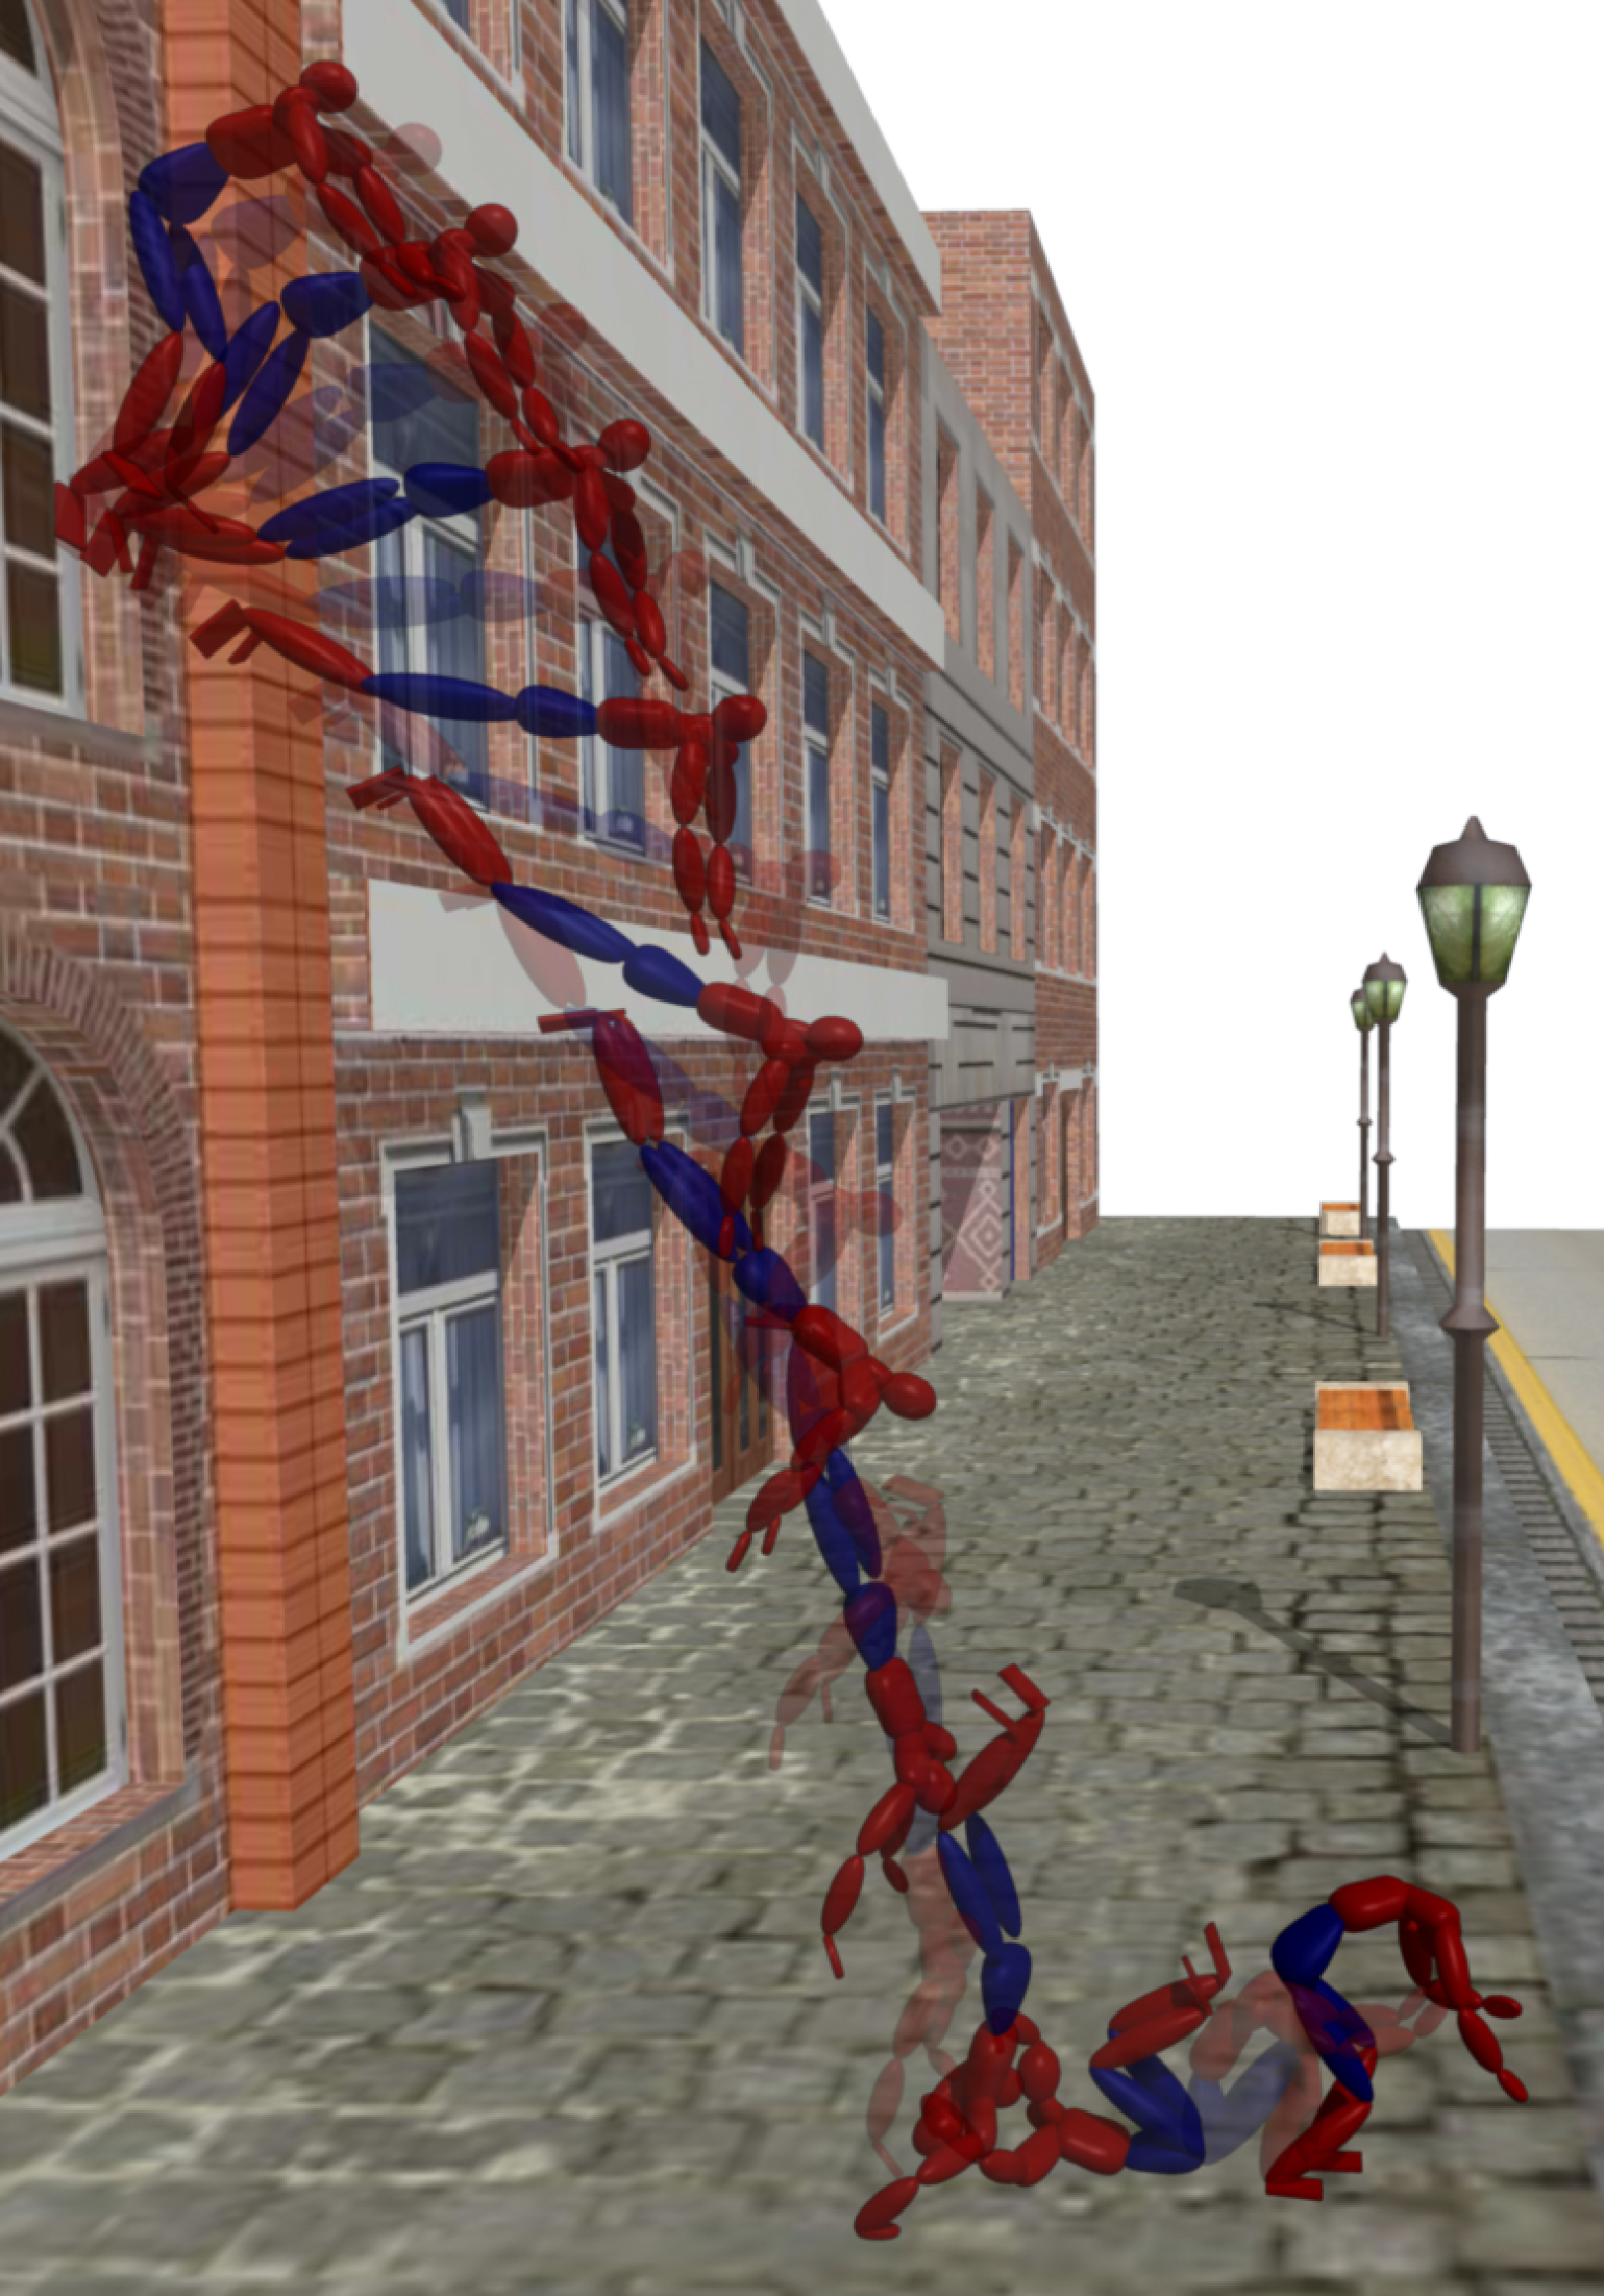
\includegraphics[width=4.0in]{images/ResultImageCol}
  \caption{Hands-first landing motion.}
  \label{fig:landing_resultHands}
\end{figure}

%% \begin{table}
%% \center
%% {
%% %% \small
%% \caption{
%%   Range of initial conditions. Top: Hands-first landing
%%   strategy. Bottom: Feet-first landing strategy.
%%   \sehoon{Statistics for success rate}
%% }
%% \begin{tabular}{|c| c|  c| c|  c| c| c|}
%% \hline
%% \label{tab:initialConditions}
%%   & {\small \textbf{y}}{\tiny(m)} 
%%   & {\small \textbf{$v_z$}}\tiny{(m/s)} 
%%   & {\small\textbf{$v_x$}}{\tiny(m/s)}  
%%   & {\small\textbf{$\omega_x$}}{\tiny(Rad/s)} 
%%   & {\small \textbf{$\omega_y$}}{\tiny(Rad/s)} 
%%   & {\small \textbf{$\omega_z$}}{\tiny(Rad/s)} \\ \hline
%% {\small \textbf{Hands: min}} & {\small 2.0 } & {\small 0.0} & {\small -1.0} & {\small 0.0} & {\small -0.5} & {\small -0.5} \\ \hline
%% {\small \textbf{Hands: max}} & {\small 10.0} & {\small 8.0} & {\small  1.0} & {\small 8.0} & {\small  0.5} & {\small  0.5} \\\hline
%% {\small \textbf{Feet: min}} & {\small 2.0 } & {\small -4.0} & {\small -4.0} & {\small -4.0} & {\small -6.0} & {\small -6.0} \\ \hline
%% {\small \textbf{Feet: max}} & {\small 10.0} & {\small  8.0} & {\small  4.0} & {\small  8.0} & {\small  6.0} & {\small  6.0} \\ \hline
%% \end{tabular}
%% }
%% \end{table}

\begin{table}
\center
{
%% \small
\caption{
  Initial conditions of the examples shown in the video (in order of appearance)
}
\begin{tabular}{| c| c|  c| c|  c| c| c|}

\hline

\multicolumn{7}{|c|}{\small Hands-first landing strategy} \\ \hline

  {\small \textbf{$\vec{C}_y$}}{\tiny(m)} 
  & {\small \textbf{$v_x$}}{\tiny(m/s)}  
  & {\small \textbf{$v_y$}}{\tiny(m/s)}  
  & {\small \textbf{$v_z$}}\tiny{(m/s)} 
  & {\small \textbf{$\omega_x$}}{\tiny(Rad/s)} 
  & {\small \textbf{$\omega_y$}}{\tiny(Rad/s)} 
  & {\small \textbf{$\omega_z$}}{\tiny(Rad/s)} \\ \hline


{\small 10.6} & {\small 0.0} & {\small 0.0} & {\small 4.0} & {\small 8.7} & {\small 0.0} & {\small 0.0} \\ \hline
{\small 5.8} & {\small 0.0} & {\small 0.0} & {\small 2.3} & {\small 5.0} & {\small 0.0} & {\small 0.0} \\ \hline
{\small 10.6} & {\small 0.0} & {\small 0.0} & {\small 6.0} & {\small 2.5} & {\small 0.0} & {\small 0.0} \\ \hline
{\small 2.5} & {\small 0.0} & {\small 0.4} & {\small 8.0} & {\small 5.0} & {\small 0.0} & {\small 0.0} \\ \hline

\hline

\multicolumn{7}{|c|}{\small Feet-first landing strategy}   \\\hline

  {\small \textbf{$\vec{C}_y$}}{\tiny(m)} 
  & {\small \textbf{$v_x$}}{\tiny(m/s)}  
  & {\small \textbf{$v_y$}}{\tiny(m/s)}  
  & {\small \textbf{$v_z$}}\tiny{(m/s)} 
  & {\small \textbf{$\omega_x$}}{\tiny(Rad/s)} 
  & {\small \textbf{$\omega_y$}}{\tiny(Rad/s)} 
  & {\small \textbf{$\omega_z$}}{\tiny(Rad/s)} \\ \hline


{\small 6.0} & {\small 0.0} & {\small 0.0} & {\small 5.0} & {\small 4.0} & {\small -1.0} & {\small -5.8} \\ \hline
{\small 2.7} & {\small 0.0} & {\small -1.0} & {\small 0.0} & {\small 0.0} & {\small 0.0} & {\small 0.0} \\ \hline
{\small 5.5} & {\small 1.0} & {\small 0.0} & {\small 0.0} & {\small 0.0} & {\small 5.0} & {\small 0.0} \\ \hline
{\small 9.6} & {\small -2.0} & {\small 0.0} & {\small -3.5} & {\small 0.9} & {\small 2.1} & {\small -3.9} \\ \hline

\end{tabular}
\label{tab:landing_initialConditions}
}
\end{table}


To evaluate the generality of our algorithm, we simulated landing
motions with a wide range of initial conditions (Table
\ref{tab:landing_initialConditions}), various landing styles (hands-first, feet-first,
consecutive rolls), and different skeleton models. We also demonstrated that
our algorithm is robust to unpredicted runtime perturbations and
different physical properties of the landing surface. Please see the
accompanying video to evaluate the quality of our results.


\paragraph{Feet-first landing strategy.} The most recommended landing
strategy from freerunning community is the feet-first landing. Our
results verify that the feet-first landing strategy is indeed very
robust for falls with arbitrary linear and angular momentum. There are
two key advantages of using feet as the first point of contact. First,
average human has longer and stronger legs than arms. Using legs to
land provides more time and strength to compress and absorb vertical
impact. Second, the feet-first strategy has an additional thrusting
step after compression and before rolling stage. During the thrusting
step, the character can utilize the contact forces to drastically
change the linear and angular velocity in preparation for rolling. Our
results show that a successful forward roll can be carried out even
when the character is falling with backward and lateral linear
velocity or nonplanar angular velocity.
%% (Figure \ref{fig:resultFeet}).

For the feet-first strategy, the coefficients of the landing condition in
Equation (\ref{eqn:landing_approxLandingAngle}) are: $a = -0.01, b = -0.06, c =
-0.03$, and $d = 0.45$. When the character transitions to the rolling
stage, we specified an asymmetric ready-to-roll pose to increase the
visual appeal of the motion.

\paragraph{Hands-first landing strategy.}
Using hands as the first point of contact can generate visually
pleasing stunts (Figure \ref{fig:landing_resultHands}). For falls with
dominant planar velocity ($v_z$ and $\omega_x$), the hands-first
strategy performs as well as the feet-first strategy. However, when
the initial condition has large lateral linear momentum or angular
momentum in yaw and roll axes, the hands-first strategy becomes less
robust. Unlike the feet-first strategy, which has an additional
thrusting step, the hands-first strategy is unable to change forward
direction drastically after landing. This imposes stringent conditions
on the contact forces because, in order to roll successfully, the
contact forces must counteract non-planner momentum, while stopping
downward momentum and maintaining forward momentum. Such forces
usually violate the unilateral constraint of ground reaction force.

For the hands-first strategy, the coefficients of the landing condition
are: $a = -0.01, b = -0.06, c = -0.03$, and $d = 3.08$. Note that the
coefficients are identical to those of the feet-first strategy except
for the constant term, indicating that the gradient of the angle of
attack with respect to the landing velocity is the same between
feet-first and hands-first landing strategies. 
%% We used a symmetric ready-to-roll pose for the hands-first strategy
%% because it reduces the chance of spinning and sideway rolling.

\paragraph{Consecutive rolls.}
Once the character starts rolling, it is rather effortless to continue
on. By looping the end of the rolling stage back to the beginning, we
showed that the character was able to make two consecutive rolls to
break a fall with large forward speed. Falling on multiple surfaces is
also easy to simulate using our controller. One example demonstrated a
continuous sequence of the character landing on the roof of a car,
leaping forward, landing again on the sidewalk, and finishing with a
dive roll (Figure \ref{fig:landing_teaser}). With our controller, a variety of
impressive action sequences can be generated easily without any
recorded or pre-scripted motions.
\begin{figure}[ht]
\center
  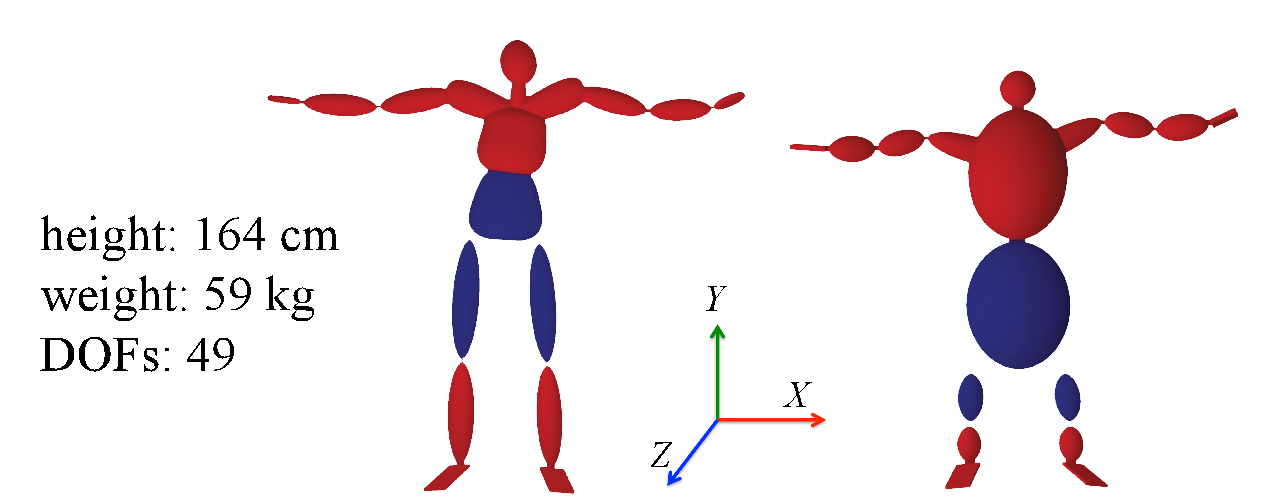
\includegraphics[width=4.2in]{images/diffSkel1}
  \caption{
    Left: The character model used for most examples. Right: A
    character with a disproportionately large torso and short legs.
  }
 \label{fig:landing_models}
\end{figure}
\paragraph{Different skeleton models.}
The character model we used to generate most examples has a height of
$164$cm, a weight of $59$ kg, and $49$ DOFs. The controllers designed
for this character can be applied to a drastically different character
whose torso is twice as long and twice as wide, comparing to the
default character. It also has very short legs and a small head
(Figure \ref{fig:landing_models}). We tested both hands-first and feet-first
landing strategies on this new character. The results are similar in
quality to the default character, although the new character hits its
head on the ground because it is difficult to tuck the head with such
a short neck.
All the control parameters remain the same for the second
character, except for $\bar{c}_y$ increasing by  $5cm$ and the
desired landing angle increasing by $0.25 rad$.


\paragraph{Runtime perturbations.}
One great advantage of physical simulation is that the outcome can be
altered on the fly based on user interactions. We demonstrated the
interactivity of our simulation in two different ways. First, the user
can directly ``drag'' the character to a different location or
orientation when the character is in the air. This example shows off
robustness and efficiency of our airborne controller. As the character
being relocated, it starts to recalculate and finds a new plan to
execute in real-time. Second, we let the user shoot cannons at the
character as a source of external forces. When a cannon hits the
character, it exerts force and torque on the character, causing a
passive response followed by active replanning and execution.

\paragraph{Different landing surfaces.}
We tested our controller on surfaces with different elasticities and
friction coefficients. When the character lands on an elastic surface,
such as a gymnastic floor or a trampoline, the character tumbles in
the air instead of rolling on the ground. We generated a continuous
sequence where the character stopped the fall on an elastic surface by
tumbling three times and finishing with a forward roll. This example
shows that various interesting acrobatic sequences can be
generated by simply concatenating our falling and rolling controllers
repeatedly. In another example, we reduced the friction coefficient to
simulate an icy surface. The character was able to use the same control
algorithm to roll, but failed to stand up at the end.

\subsection{Evaluation}

\paragraph{Performance.}
All the results shown in the video were produced on a single core of
3.20GHz CPU. Our program runs at $550$ frames per second. The
bottleneck of the computation is the optimization routine in the
airborne controller. We use Open Dynamic Engine to simulate the
character. The time step is set at $0.2$ millisecond, and runs
the airborne optimization in 50 Hz.
\begin{figure}[ht]
\center
  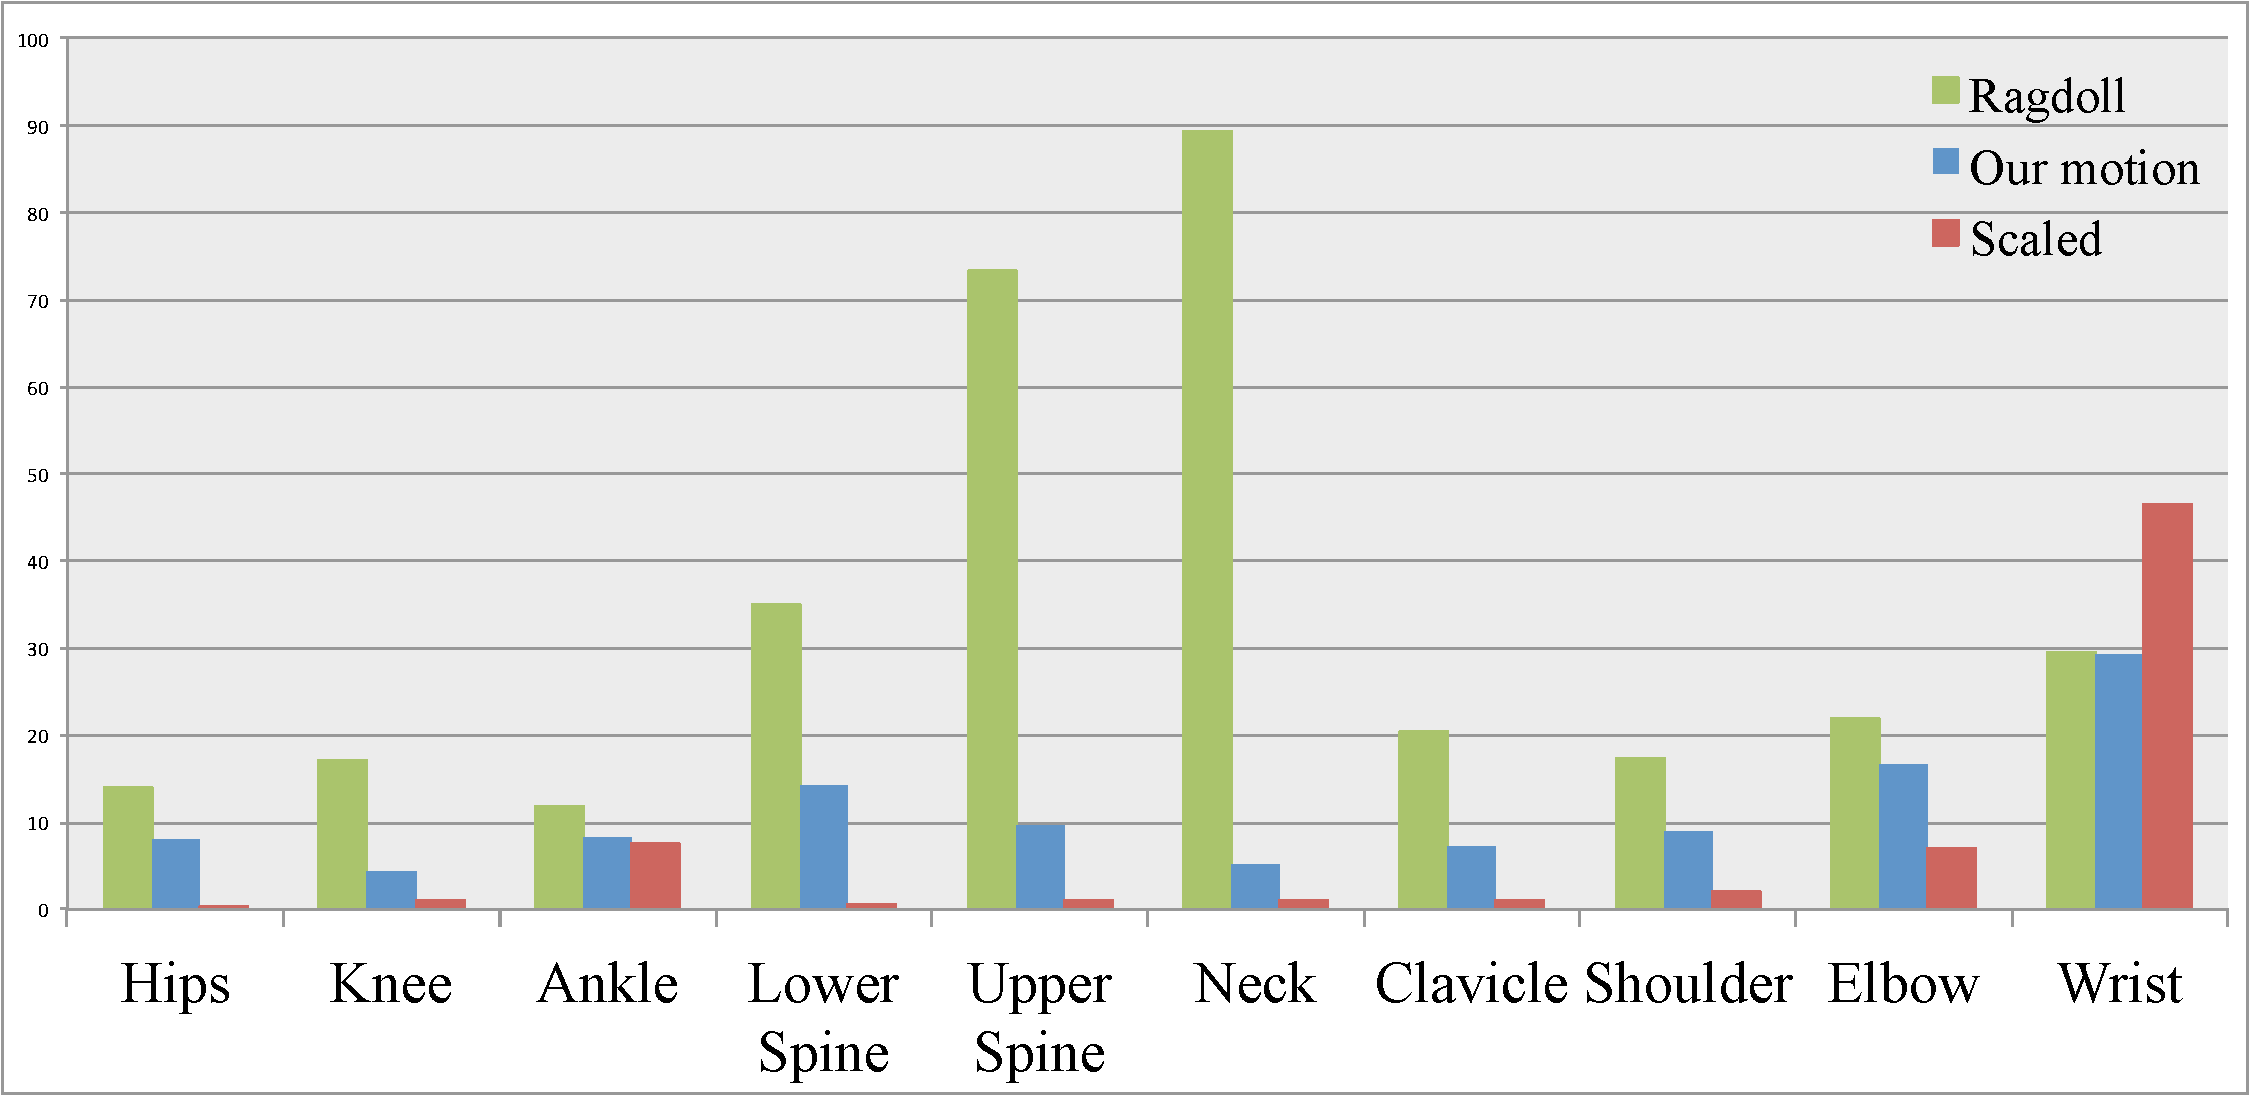
\includegraphics[width=4.2in]{images/stress}
  \caption{
    Maximal stress for each joint from a hands-first landing
    motion. Results are quantitatively similar across all of our
    simulations. Green: Ragdoll motion. Blue: Our motion. Orange: Joint
    stress scaled by mass.}
%% \karen{Order of three bars: Green, blue,
%%       and orange. The joint names from left to right: Hip, Knee,
%%       Ankle, Lower spine, Upper spine, Neck, Clavicle, Shoulder,
%%       Elbow, and Wrist.}
 \label{fig:landing_jointStress}
\end{figure}
\paragraph{Joint stress.}
We approximated joint stress as the constraint force that holds two
rigid bodies together at a joint. For each joint, we computed the
maximal joint stress during the landing phase (Figure
\ref{fig:landing_jointStress}). We observed that, in most trials, the joints
which endure the most impact are those connected to contacting
end-effectors (\ie hands or feet). The spine joints (lumbar and
thoracic vertebrae) and hip joints are also subject to large
impact. However, when we scaled each joint by the total mass it
supports (\eg the hip joint supports the mass of the entire leg), we
found that the joint stress has low variance across the entire
character's body, with the exception of the joints near the
end-effectors.
%% \begin{table}
%% \center
%% {
%% %% \small
%% \caption{Joint Stress Comparison}

%% \begin{tabular}{c  c c}
%% \label{tab:jointStress}
%%  } & \textbf{Ragdoll} & \textbf{Our controller} \\ \hline

%% \textbf{Neck}     & 73.26 &  9.74   \\ \hline
%% \textbf{Spine}    & 35.09 & 14.14   \\ \hline
%% \textbf{Shoulder} & 20.30 &  7.35   \\ \hline
%% \textbf{Hips}     & 13.98 &  7.91   \\ \hline
%% \end{tabular}
%% }
%% \end{table}


When we compared the joint stress between our motion and a passive
ragdoll motion with the same initial condition, the ragdoll motion
caused much more damage on the neck and the spine (Figure
\ref{fig:landing_jointStress}). In fact, the only joints that endured similar
amount of stress were those used for the first point of contact (\eg
wrists or ankles). These results validate that our controller indeed
produces safer landing motion and protects important body parts. We
repeated the experiments for different initial conditions.  In the
worst case of our experiments, the average joint stress is still four
times lower than landing as a passive ragdoll. The data also show that
our controller generates less damaging landing motion even when the
character cannot roll successfully, such as dropping from $20$ meters.


\paragraph{Comparison with video footages.}
We compared our simulated motion side-by-side with a collection of
video footages (\cite{APR:2011:URL}).  The simulations are based on the
same landing strategy and our best guess of the initial conditions from
the videos. Although it is not possible to achieve identical motions,
results show that our motion is qualitatively similar to the video
footages.

\subsection{Limitations}
The main limitation of our work is the lack of balance control after
the character stands up. There are many existing balance control
algorithms we could implement. However, we chose to defer the
implementation until we decide on what the character's next action
should be. In the freerunning scenario, the character transitions to
running motion seamlessly right after a roll. If freerunning is our goal, we
would modify the current get-up control algorithm to provide more
forward thrust. Other possibilities of the next action include
walking, stepping, jumping, or standing still. Different next actions
will result in different balance strategies. Ideally, a character
should be equipped with motor skills to execute all different balance
strategies and autonomously determines which strategy to execute, but
this is considered out of the scope of this work.

Another limitation is the predefined landing pose for each landing
strategy. This inflexibility can negatively affect the character's
ability to adapt to different environments. For example, if the
character lands on a narrow wall, the landing pose needs to be
adjusted on the fly. One possible solution is to use a simple inverse
kinematics method to compute desired joint angles before landing.



\begin{figure}[ht]
\center
  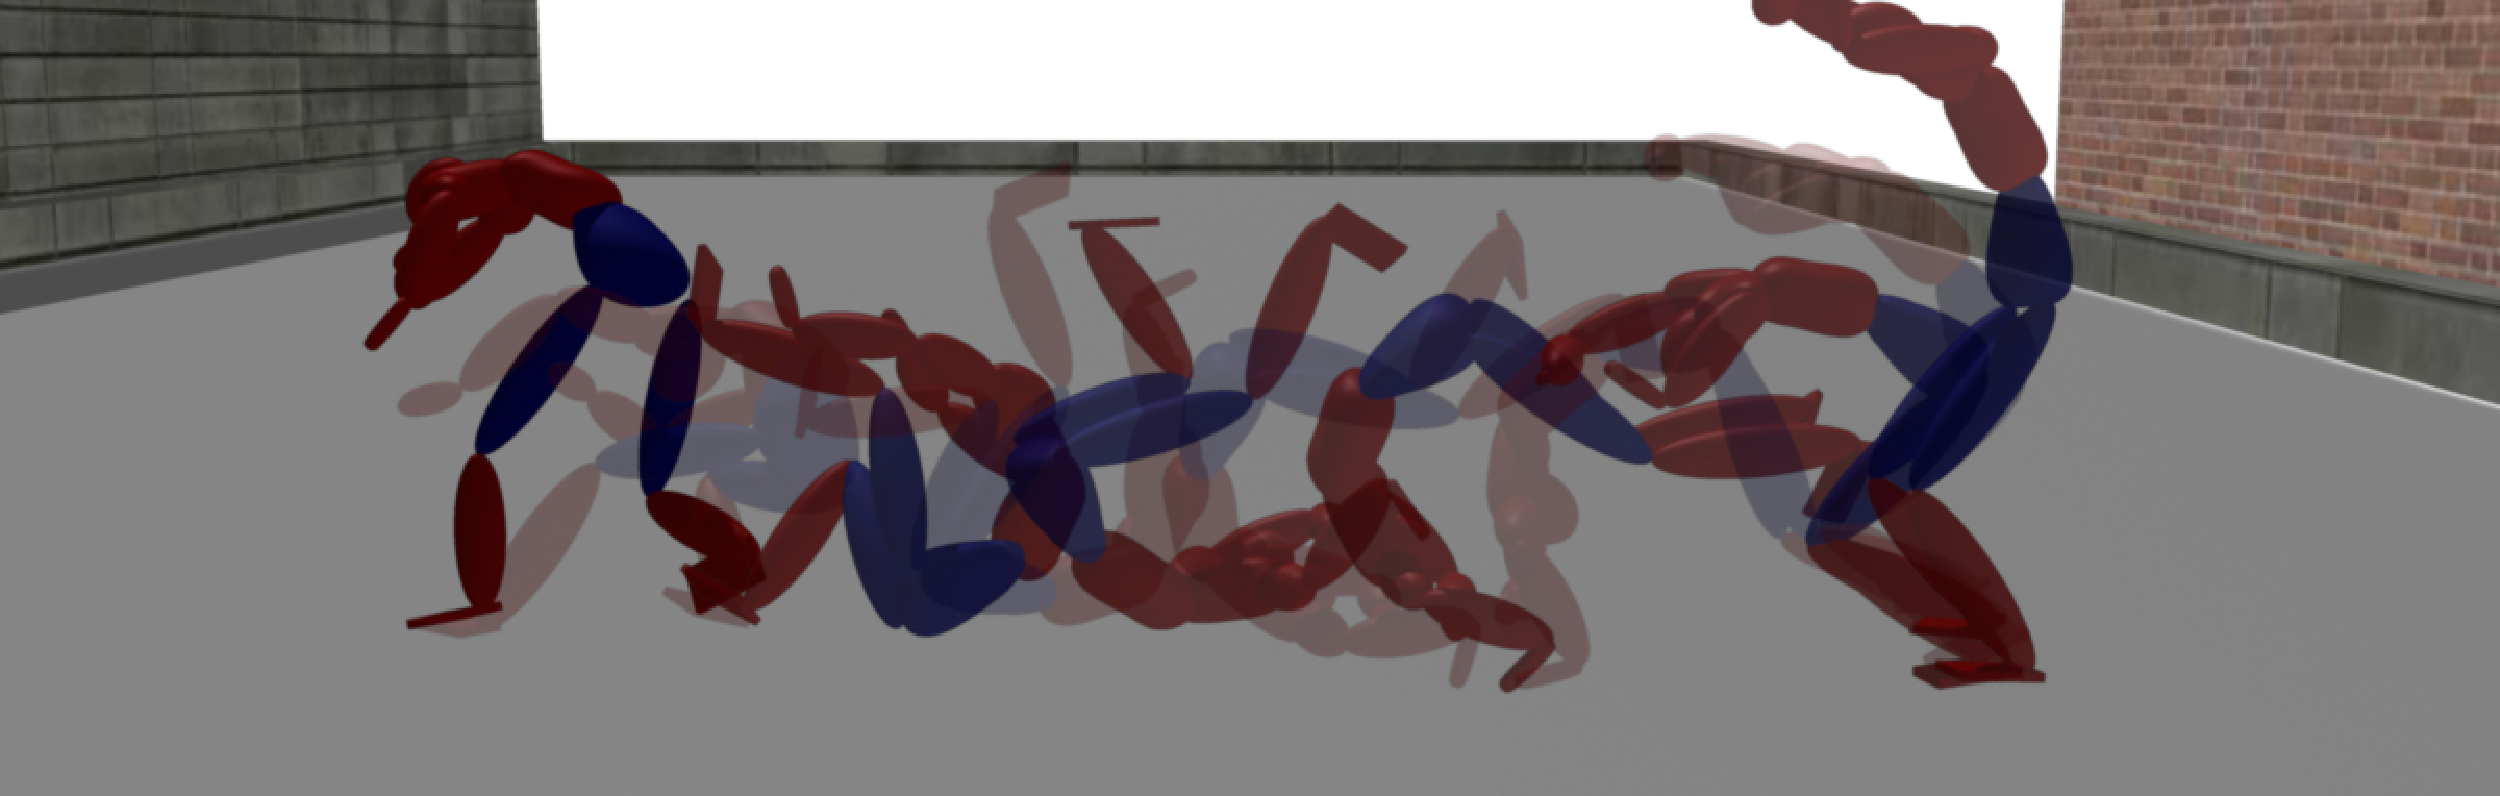
\includegraphics[width=0.95\textwidth]{images/ResultRoll}
  \caption{Feet-first landing motion.}
  \label{fig:landing_resultFeet}

\end{figure}

\section {Discussion}

We introduced a real-time physics-based technique to simulate
strategic falling and landing motions. 
Our control algorithm reduces
joint stress due to landing impact and allows the character to
efficiently recover from the fall.
 Given an arbitrary initial position
and velocity in the air, our control algorithm determines an
appropriate landing strategy and an optimal sequence of actions to
achieve the desired landing velocity and angle of attack. The
character utilizes virtual forces and joint-tracking control
mechanisms during the landing phase to successfully turn a fall into a
roll. We demonstrated that our control algorithm is general,
efficient, and robust by simulating motions from different initial
conditions, characters with different body shapes, different physical
environments, and scenarios with real-time user perturbations.  The
algorithm guides the character to land safely without introducing the
large stress at every joint except for the contacting end-effectors.

Freerunning is a great exemplar to demonstrate human athletic
skills. Those wonderfully simple yet creative movements provide a
rich domain for future research directions. Based on the contribution
of this work, we would like to explore other highly dynamic skills in
freerunning, such as cat crawl, underbar, or turn vault. These motions
are extremely interesting and challenging to simulate because they
involve sophisticated planning and control in both cognitive and motor
control levels, as well as complex interplay between the performer and
the environment.

The landing strategies described in this work are suitable for highly
dynamic activities, but not optimal for low-clearance falls from
standing height. There is a vast body of research work in biomechanics
and kinesiology studying fall mechanics of human from standing
height. One future direction of interest is to integrate this domain
knowledge with physical simulation tools to explore new methods for
fall prevention and protection.


